\documentclass[11pt]{article}
% paragraph spacing

\usepackage{amsmath, amsfonts, amssymb, graphicx}
\usepackage[round]{natbib}
\usepackage{dsfont}
\usepackage{mathtools}
\usepackage{framed}
\usepackage{listings}
\usepackage{subcaption}
\usepackage[margin=1.0in]{geometry}
\usepackage{float}
\usepackage{hyperref}
\usepackage{rotating}

\lstset{breaklines=true}
\lstset{basicstyle=\ttfamily}
\setlength{\parskip}{6pt}

\newcommand{\impmark}{\strut\vadjust{\domark}}
\newcommand{\domark}{%
  \vbox to 0pt{
    \kern-\dp\strutbox
    \smash{\llap{$\rightarrow$\kern1em}}
    \vss
  }%
}

\begin{document}
\bibliographystyle{sysbio}
\bibpunct[; ]{(}{)}{;}{a}{}{;}

\title{Biogeographic dating in RevBayes}
\author{Michael J. Landis \\ \href{mailto:mlandis@berkeley.edu}{\texttt{mlandis@berkeley.edu}}}
\maketitle

\section{Introduction}

This lab describes how to jointly infer the posterior range evolution parameters, ancestral ranges, and divergence times using RevBayes.
%BayArea is a C++ command-line program that implements the method described in \citet{landis13}.
Phylowood is a Javascript web service that for animating and filtering phylogenetic biogeographic reconstructions \citep{landis14}. \\

\noindent \textbf{By the end of this lab you should know how to} \\
- Describe how the model and method \\
- Identify the data needed for a biogeographic dating analysis \\
- Configure and run an MCMC analysis \\
- Review the MCMC tracer file \\
- Retrieve posterior ancestral range reconstructions \\
- Generate a Phylowood animation

\noindent \\ \impmark These little arrows indicate lines containing key information to progress through the lab. The rest of the text gives context for why we're taking these steps or what to make of results.

\subsection{Handy links for this lab}

\begin{tabular}{ll}
Lab zip file & \url{http://treethinkers.org/wp-content/uploads/2014/03/bayarea_lab.zip} \\
Phylowood software & \url{http://mlandis.github.io/bayarea-fig} \\
Phylowood manual & \url{https://github.com/mlandis/phylowood/wiki} \\
DendroPy manual & \url{http://pythonhosted.org/DendroPy/} \\
matplotlib manual & \url{http://matplotlib.org/} \\
NumPy manual & \url{http://www.numpy.org/}

\end{tabular}

\subsection{Setting up your workspace}

The practical part of the lab will analyze the simulated dataset we just reviewed.
Parts of the lab will require entering terminal commands, which will assume you are using the Unix shell \texttt{bash}.
Just ask for help if the commands don't seem to work.

\noindent \\ \impmark Portions of this lab require Python is installed, along with the Dendropy, matplotlib, and NumPy packages.

\noindent \\ \impmark This tutorial will assume you have successfully installed BayArea to the directory \newline{\texttt{\char`\~/apps/bayarea\_1.0.2/}}. Shell commands will assume this is your current working directory.

\noindent \\ \impmark Download and unzip the lab zip file, \texttt{bayarea\_lab.zip}, into \texttt{\char`\~/apps/bayarea\_1.0.2}.

\noindent \\ \impmark Copy all files into \texttt{./examples/}

\begin{framed}
\begin{lstlisting}
> ls bayarea_lab
my_data.txt                 my_run.area_states.txt
my_geo.txt                  my_run.nhx
my_lab_run.sh               my_run.parameters.txt
my_other_run.parameters.txt my_tree.txt
my_run.area_probs.txt       pp_range.py

> cp bayarea_lab/* ./examples
\end{lstlisting}
\end{framed}

\noindent \\ \impmark Move the shell script, \texttt{my\_lab\_run.sh}, into the main app directory, and set the file to be executable

\begin{framed}
\begin{lstlisting}
> mv examples/my_lab_run.sh .
> chmod 766 my_lab_run.sh
\end{lstlisting}
\end{framed}

\section{Model and method}

This section contains a brief description of the data, model, parameters, and method used in BayArea.

First, we define the range for taxon $i$ as the bit vector $X_i$, where $X_{i,j} = 1$ if the taxon is present in area $j$ and $X_{i,j} = 0$ if the taxon is absent.
Each taxon range is a bit vector of length $N$ areas.
For example, if taxon $B$ is present only in areas 2 and 3 out of $N=3$ areas, its range is represented as $X_B = (0,1,1)$, which is translated to the bit string $X_B=011$ for short.
The data matrix, $\textbf{X}$, is analogous to a multiple sequence alignment where each element in the data matrix reports a discrete value for a homologous character shared by all taxa at column $j$.
How to choose areas to define species ranges will not be covered in this tutorial.

Next, we need a model of range evolution.
Since we have discrete characters we'll use the continuous-time Markov chain, which allows us to compute transition probability of a character changing from $i$ to $j$ in time $t$ through matrix exponentiation
\[
\mathbf{P}_{i,j}(t) = \left[ \exp \left\lbrace \mathbf{Q}t \right\rbrace \right]_{i,j},
\]
where $\textbf{Q}$ is the instantaneous rate matrix defining the rates of change between all pairs of characters, and $\textbf{P}$ is the transition probability rate matrix.
This technique of matrix exponentiation is powerful because it integrates over all possible scenarios of character transitions that could occur during $t$ so long as the chain begins in state $i$ and ends in state $j$.

We can then encode range evolution events into the allowed character transitions of $\textbf{Q}$ and parameterize the events so that we may infer their relative importance to generating our observed ranges.
We'll take a simple model of range expansion (e.g. $011 \rightarrow 111$) and range contraction (e.g. $011 \rightarrow 001$).
(Range expansion may also be referred to as dispersal or area gain and range contraction as extirpation or area loss.)
The rates in the transition matrix for three areas might appear as

\[
\textbf{Q} = 
	\begin{array}{r|cccccccc}
		& 000 & 001 & 010 & 011 & 100 & 101 & 110 & 111 \\
		\hline
		000 & - & 0 & 0 & 0 & 0 & 0 & 0 & 0 \\
		001 & \lambda_0 & - & 0 & \lambda_1 & 0 & \lambda_1 & 0 & 0 \\
		010 & \lambda_0 & 0 & - & \lambda_1 & 0 & 0 & \lambda_1 & 0 \\
		011 & 0 & \lambda_0 & \lambda_0 & - & 0 & 0 & 0 & \lambda_1 \\
		100 & \lambda_0 & 0 & 0 & 0 & - & \lambda_1 & \lambda_1 & 0 \\
		101 & 0 & \lambda_0 & 0 & 0 & \lambda_0 & - & 0 & \lambda_1 \\
		110 & 0 & 0 & \lambda_0 & 0 & \lambda_0 & 0 & - & \lambda_1 \\
		111 & 0 & 0 & 0 & 0 & \lambda_0 & \lambda_0 & \lambda_0 & - \\								
	\end{array},
\]
which can also be represented compactly as the rate function
\[
q^{(a)}_{\textbf{y},\textbf{z}} =
\begin{cases}
\lambda_0 & \text{if $z_a=0$}  \\
\lambda_1 & \text{if $z_a=1$} \\
0 & \mathbf{y} = 00...0 \\
0 & \text{\textbf{y} and \textbf{z} differ in more than one area}
\end{cases},
\]
where $\textbf{y}$ and $\textbf{z}$ are the ``from'' and ``to'' ranges and $a$ is the area that changes.
For example, $q^{(1)}_{011,111}$ is the rate of range expansion for $011 \rightarrow 111$ to gain area $1$.
Since the taxon is extinct for the entirely unoccupied range, $00...0$, its rate of range expansion is zero (barring resurrection).
Also note the rate of more than one event occurring simultaneously is zero.

However, we may reasonably expect that a range expansion event into an area depends on which nearby areas are currently inhabited.
The transition rate might then appear as
\[
q^{(a)}_{\textbf{y},\textbf{z}} =
\begin{cases}
\lambda_0 & \text{if $z_a=0$}  \\
\lambda_1 \eta(\textbf{y}, \textbf{z}, a, \beta) & \text{if $z_a=1$} \\
0 & \mathbf{y} = 00...0 \\
0 & \text{\textbf{y} and \textbf{z} differ in more than one area}
\end{cases}.
\]
The behavior of $\eta(\cdot)$ is given in finer detail in \citet{landis13}.
For this tutorial, you can take $\eta(\cdot)$ to adjust the rate of range expansion into area $a$ by considering how close it is to the current range, $\textbf{y}$ relative to the closeness of all other areas unoccupied by the taxon.
The $\beta$ parameter rescales the importance of geographic distance between two areas by a power law.
Importantly, $\eta(\cdot) = 1$ when $\beta=0$, meaning geographic distance between areas is irrelevant.
Moreover, when $\beta > 0$, $\eta(\cdot) < 1$ when area $a$ is relatively distant and $\eta(\cdot) > 1$ when area $a$ is relatively close.

Let's consider what happens to the size of \textbf{Q} when the number of areas, $N$, becomes large.
For three areas, \textbf{Q} is size $8 \times 8$.
For ten areas, \textbf{Q} is size $1024 \times 1024$, which approaches the largest size matrix that can be exponentiated in a practical amount of time.
This is problematic, meaning we need an alternative method to integrate over historical range evolution events.

You may wonder why matrix exponentiation works fine for molecular substitution models and large multiple sequence alignments.
Because recombination degrades linkage disequilibrium over geological timescales, molecular substitution models typically assume each site in the multiple sequence alignment evolves independently.
Conveniently, this keeps \textbf{Q} small even for datasets with many sites.

Remember matrix exponentiation integrates over all \textit{unobserved} transition events during time $t$.
The likelihood of beginning in character $i$ and ending in character $j$ can be computed easily when the explicit series of event types and times are known.
While we will never know the exact history of events, we can use stochastic mapping in conjunction with Markov chain Monte Carlo (MCMC) to repeatedly sample range evolution histories that are consistent with the ranges observed in the study taxa at the tips of the phylogeny.

This is the strategy used in BayArea to infer the posterior distribution approximated is 
\newline{Prob$\left( \textbf{X}_{aug}, \theta \mid \textbf{X}_{obs}, T, M \right)$}, where $\textbf{X}_{obs}$ is the range data observed at the tips, $\textbf{X}_{aug}$ is the distribution of ancestral range reconstructions over the phylogeny, $T$, where $\textbf{X}_{aug}$ is inferred jointly with the parameters, $\theta$, assuming the range evolution model, $M$, that describes $\textbf{Q}$ above.
Ancestral range reconstructions are often of primary interest in phylogenetic biogeographic analyses, which are generated with support values as a by-product of the MCMC analysis.

The rest of the tutorial will describe how to assemble the input, run the analysis, assess the output, and visualize the results.

\section{Lab Outline}

%1) Pre-analysis
%1.a) Format data partitions. \\
%1.b) Infer MAP topology, T. \\
1) Pre-analysis
2) Biogeographic calibration analysis
2.a) Format data partitions. \\
2.a) Define geography. \\
2.c) Infer joint posterior over molecular data, range data, and divergence times given T. \\
3) Review results. \\
3.a) Parameter output \\
3.b) Ancestral range output \\
3.c) Visualize ancestral range reconstructions. \\

\section{Input}

This section describes how to generate the files needed for biogeographic calibration analysis.

As an example, we'll use a dataset for 19 species of $Psychotria$ whose range spans the Hawaiian archipelago.
. originated from \cite{XXX} 
The model will assume presence-absence characters are recorded without error.
Areas are defined over the Hawaiian archipelago in numbers that 

\subsection{Pre-analysis}
The biogeographic calibration analysis described in this tutorial assumes the tree topology is known.
For this, you'll need the Newick string for {\it e.g.} a {\it maximum a posterior} (MAP) topology or most credible clade (MCC) topology, which can be generated by following other RevBayes, MrBayes, or BEAST tutorials.
Generally, you will want to use the molecular data from that analysis for the divergence time estimation.

\noindent \\ \impmark Open the file \texttt{examples/my\_tree.txt}.

\begin{framed}
\begin{lstlisting}
(((((t1:1.040892,(t2:0.024898,t3:0.024898):1.015994):0.637439,((t4:0.379109,t5:0.379109):1.158215,t6:1.537324):0.141007):0.428946,((t7:0.26996,t8:0.26996):0.535304,t9:0.805264):1.302013):0.723986,
...
\end{lstlisting}
\end{framed}

Because range evolution occurs in units of geological time, a BayArea analysis requires a high-quality time-calibrated phylogeny. This typically requires a multiple sequence alignment over several loci plus fossils for calibration.
Since this data availability is often the limiting factor for which taxa to include for your analysis, it is best to produce the phylogeny first.
Only afterwards should you begin assembling data for your data matrix.
%Tracy Heath has an excellent tutorial on how to generate time calibrated trees (\href{.
If your phylogeny cannot be calibrated (e.g. it has no fossils) your best alternative is to proceed with a time tree resulting from a divergence time estimation analysis.
For this tutorial, the phylogeny is assumed to contain no uncertainty.

\subsection{Data}

The data file contains a matrix of binary characters corresponding to the observed ranges of the study taxa.

\noindent \\ \impmark  Open the file \texttt{examples/psychotria\_range.txt}.

\begin{framed} \begin{lstlisting}
#NEXUS

begin data;
  dimensions ntax=19 nchar=4;
  format datatype=standard symbols = "01";
  matrix
    P_fauriei2          0100
    P_grandiflora_Kal2  1000
    ...
    P_wawraeDL7428      1000	
  ;
end;

Begin trees;
	TREE tree1 = ((((((((P_hawaiiensis_WaikamoiL1:1.0853
	,P_mauiensis_Eke:1.0853)N2:0.7964,(P_fauriei2:1.3826,
	P_hathewayi_1:1.3826)N5:0.4991)N6:0.1986,(
	...
	2.6568)N33:0.5204,P_hexandra_Oahu:3.1772)N35:2.6659)N36;
End;
\end{lstlisting}
\end{framed}

Range data is stored in standard Nexus format.
In the \texttt{begin data} block, the first line gives the dimensions of the data matrix and the second line indicates we will be using binary characters. 
Rows in the \textttt{matrix} block correspond to taxa and their range data, while columns give in which areas each taxon is present (1) or absent (0).
For example, taxon \texttt{P_fauriei2} is present only in area 2, which will be defined by the Geography file.

\subsection{Geography}

This model will use discrete-state biogeographic ranges, meaning the range
Each area is assigned a point to represent its geographical coordinates.
The distances between these coordinates inform to distance-dependent dispersal parameter for range expansion events.
Coordinates close to the center of the area suffice.
The first line is used to indicate the time the distances apply to and should be set to ``\# 0.0''.
Each remaining line reports the latitude and longitude in order of the areas in the columns of the data matrix.

\noindent \\ \impmark Open the file \texttt{examples/my\_areas.txt}.

\begin{framed}
\begin{lstlisting}

{
  "name":"HawaiianArchipelago10my",
  "epochs":
  [{
    "name":"epoch1",
    "start_age":10.0,
    "end_age":0.0,
    "areas":
      [{ "name": "Kauai",  "latitude":22.0833, "longitude": -159.5000, "dispersalValues": [ 1,1,1,1 ] },
       { "name": "Oahu",   "latitude":21.4722, "longitude": -157.9772, "dispersalValues": [ 1,1,1,1 ] },
       { "name": "Maui",   "latitude":20.8000, "longitude": -156.3333, "dispersalValues": [ 1,1,1,1 ] },
       { "name": "Hawaii", "latitude":19.5667, "longitude": -155.5000, "dispersalValues": [ 1,1,1,1 ] }]
  }]
}
\end{lstlisting}
\end{framed}

\section{Analysis}

\subsection{Simulated data}

The zip file contains a simulated dataset for 50 taxa over 33 terrestrial areas throughout Australia.
The rate of range expansion, rate of range contraction, and distance power parameter were set as 0.1, 0.7, and 4.0 respectively.
Additionally, the zip file contains the output from two completed MCMC analyses under the settings given below.

\subsection{Settings}

BayArea accepts command-line arguments to set input and output files, set MCMC sampling behavior, configure prior values, etc.
To reduce the risk of typos, you can execute the command with arguments using a pre-defined shell script.
For this lab, we'll be using \texttt{my\_lab\_run.sh}, which was used to produce the output files from the input files contained in \texttt{bayarea\_lab.zip}.
Before running our job, let's review the program settings by opening \texttt{my\_lab\_run.sh} using your favorite text editor.

\noindent \\ \impmark Enter the following command.
\begin{framed}
\begin{lstlisting}
> cat my_lab_run.sh
./bayarea -areaFileName=my_data.txt \
          -geoFileName=my_geo.txt \
          -treeFileName=my_tree.txt \
          -inputFilePath=./examples/ \
          -outputFilePath=./examples/ \
          -outputTimestamp=T \
          -outputPrefix=my_run \
          -parameterSampleFrequency=1000 \
          -historySampleFrequency=10000 \
          -printFrequency=10000 \
          -chainLength=50000000 \
          -chainBurnIn=0 \
          -probBurnIn=10000000 \
          -modelType=3 \
          -gainPrior=0.1 \
          -lossPrior=0.1 \
          -distancePowerPrior=0.1 \
          -guessInitialRates=T \
          -geoDistancePowerPositive=T \
          -geoDistanceTruncate=F \
          -areaProposalTuner=0.1
\end{lstlisting}
\end{framed}

The first set of flags concerns file handling.
\texttt{inputFilePath} indicates where to find the input files \texttt{areaFileName}, \texttt{geoFileName}, and \texttt{treeFileName}.
\texttt{outputFilePath} indicates where output files will be stored, which may be prefixed with \texttt{outputPrefix} and timestamped with \texttt{outputTimestamp}, both useful for organizing output from many analyses.

The second set of flags concerns the MCMC analysis length, chain burn-in, and the sampling interval.
MCMC starts at an arbitrary state (sampled from the prior) and takes some amount of time to converge to stationarity.
Once at stationarity, independent samples of the MCMC state at regular intervals approximate the target posterior distribution.
MCMC that relies on stochastic mapping for data augmentation takes a longer time to mix, because it takes many MCMC proposals to explore the space of stochastically mapped range evolution histories.
Unfortunately, you typically do not know how long it takes to reach stationarity, so it's best to run MCMC analyses for an excessive length.
\texttt{chainBurnIn} determines which cycle to begin recording the MCMC state, but generally you wish to save the entire chain and assess burn-in after the analysis.

In the next section, you'll see \texttt{my\_run.area\_probs.txt} and \texttt{my\_run.nhx} report ancestral range reconstruction probabilities.
The MCMC records the sampled histories every \texttt{historySampleFrequency} iteration to \texttt{my\_run.area\_states.txt}.
However, this data is relatively ``raw'' and must be manipulated with scripts for immediate use (we will cover how to do so later).
The probabilities in the files above are computed as part of the analysis for your convenience, disregarding the first \texttt{probBurnIn} iterations of the MCMC.
(Here it is set to disregard the first quarter of the chain.)

Parameters are sampled every \texttt{parameterSampleFrequency} iterations. The current MCMC state is printed on-screen every \texttt{printFrequency} iterations.

The final set of flags concerns model parameters.
The area gain rate ($\lambda_1$), area loss rate ($\lambda_0$), and distance power parameter ($\beta$) are each assigned their own half-Cauchy prior distribution.
The half-Cauchy distribution can be thought of as the absolute value of ``fat-tailed'' normal distributions, with scale parameters set by \texttt{gainPrior}, \texttt{lossPrior}, and \texttt{distancePowerPrior}.
The flag \texttt{guessInitialRates} makes a very rough estimate of the initial values for $\lambda_0$ and $\lambda_1$ from the data and tree rather than sampling their values from the prior distribution.
\texttt{areaProposalTuner} controls the expected proportion of areas to update during a range history proposal.
Mixing suffers when this value is too large.

The distance power parameter, $\beta$, effectively rescales the distance between areas.
When computing the probability of range expansion, the pairwise distances are computed between each occupied area in the starting range and each unoccupied area in the expanded range.
For large numbers of areas ($N > 100$), this computation can become slow.
Assigning \texttt{geoDistanceTruncate} to \texttt{T} tells the software to skip computing pairwise distances for areas that are very distant given the current value of $\beta$, i.e. areas that have an exceedingly small chance of being gained.
This speeds up computation but may introduce negligible amounts of error into computing the distance-dependent rate-modifier term, $\eta$.

Finally, there is nothing mathematically to prevent $\beta$ from becoming negative, for which range expansion events would prefer distant areas to nearby areas.
In some cases, BayArea will infer $\beta<0$ and generate implausible ancestral range reconstructions, particularly for globally distributed taxa.
So, the flag \texttt{geoDistancePowerPositive} constrains $\beta \geq 0$ when set to \texttt{T}.

See Section 4.1 of the BayArea v1.0.2 manual to learn about additional input, output, and analysis settings.

\subsection{Running a job}

Executing the shell script will run our job. Bombs away!

\noindent \\ \impmark Enter the following command.
\begin{framed}
\begin{lstlisting}
> ./my_lab_run.sh
\end{lstlisting}
\end{framed}

\section{Output}

Instead of waiting for the MCMC to finish, we'll use the output from a completed analysis on the same data.

\noindent \\ \impmark Press \texttt{ctrl-C} to kill the job.

\subsection{Screen}

There are three types of MCMC proposals, the first being parameter proposals that act upon the model parameters, $\lambda_0$, $\lambda_1$, and $\beta$.
The second type of proposals act upon our sampling parameters, $\lambda^*_0$ and $\lambda^*_1$, which we use to sample range histories but do not directly affect our model likelihood.
The last type, ancestral range history updates, occur in very high proportion to all other updates.

Recall from the Introduction that this is necessary to effectively integrate over all ancestral ranges of moderate to high posterior probability.
The screen output reports whether the proposal for that iteration was accepted or rejected.
If you notice the MCMC is rejecting most proposals, it will probably not produce an accurate approximation of the posterior.
Pay particular attention to range history proposals.
Range history proposals tend to introduce very small differences to the likelihood so they are generally accepted easily.
If you notice very few range history proposals are accepted, you will improve the acceptance probability by reducing the \texttt{areaProposalTuner} value.

\subsection{Sampled parameters (\texttt{my\_run.parameters.txt})}

This tab-delimited file contains the parameters sampled at regular intervals from the MCMC (set by \texttt{parameterSampleFrequency}).
Open the \texttt{my\_run.parameters.txt} in Tracer.
First, we see the effective sample size is only moderate for $50 \times 10^6$ cycles when sampling every 1000 cycles.
This is because the vast majority of MCMC updates are range history updates.

\noindent \\ \impmark  Highlight the ``gain'' and ``loss'' parameters then click Joint-Marginal.

\begin{figure}[H]
\centering
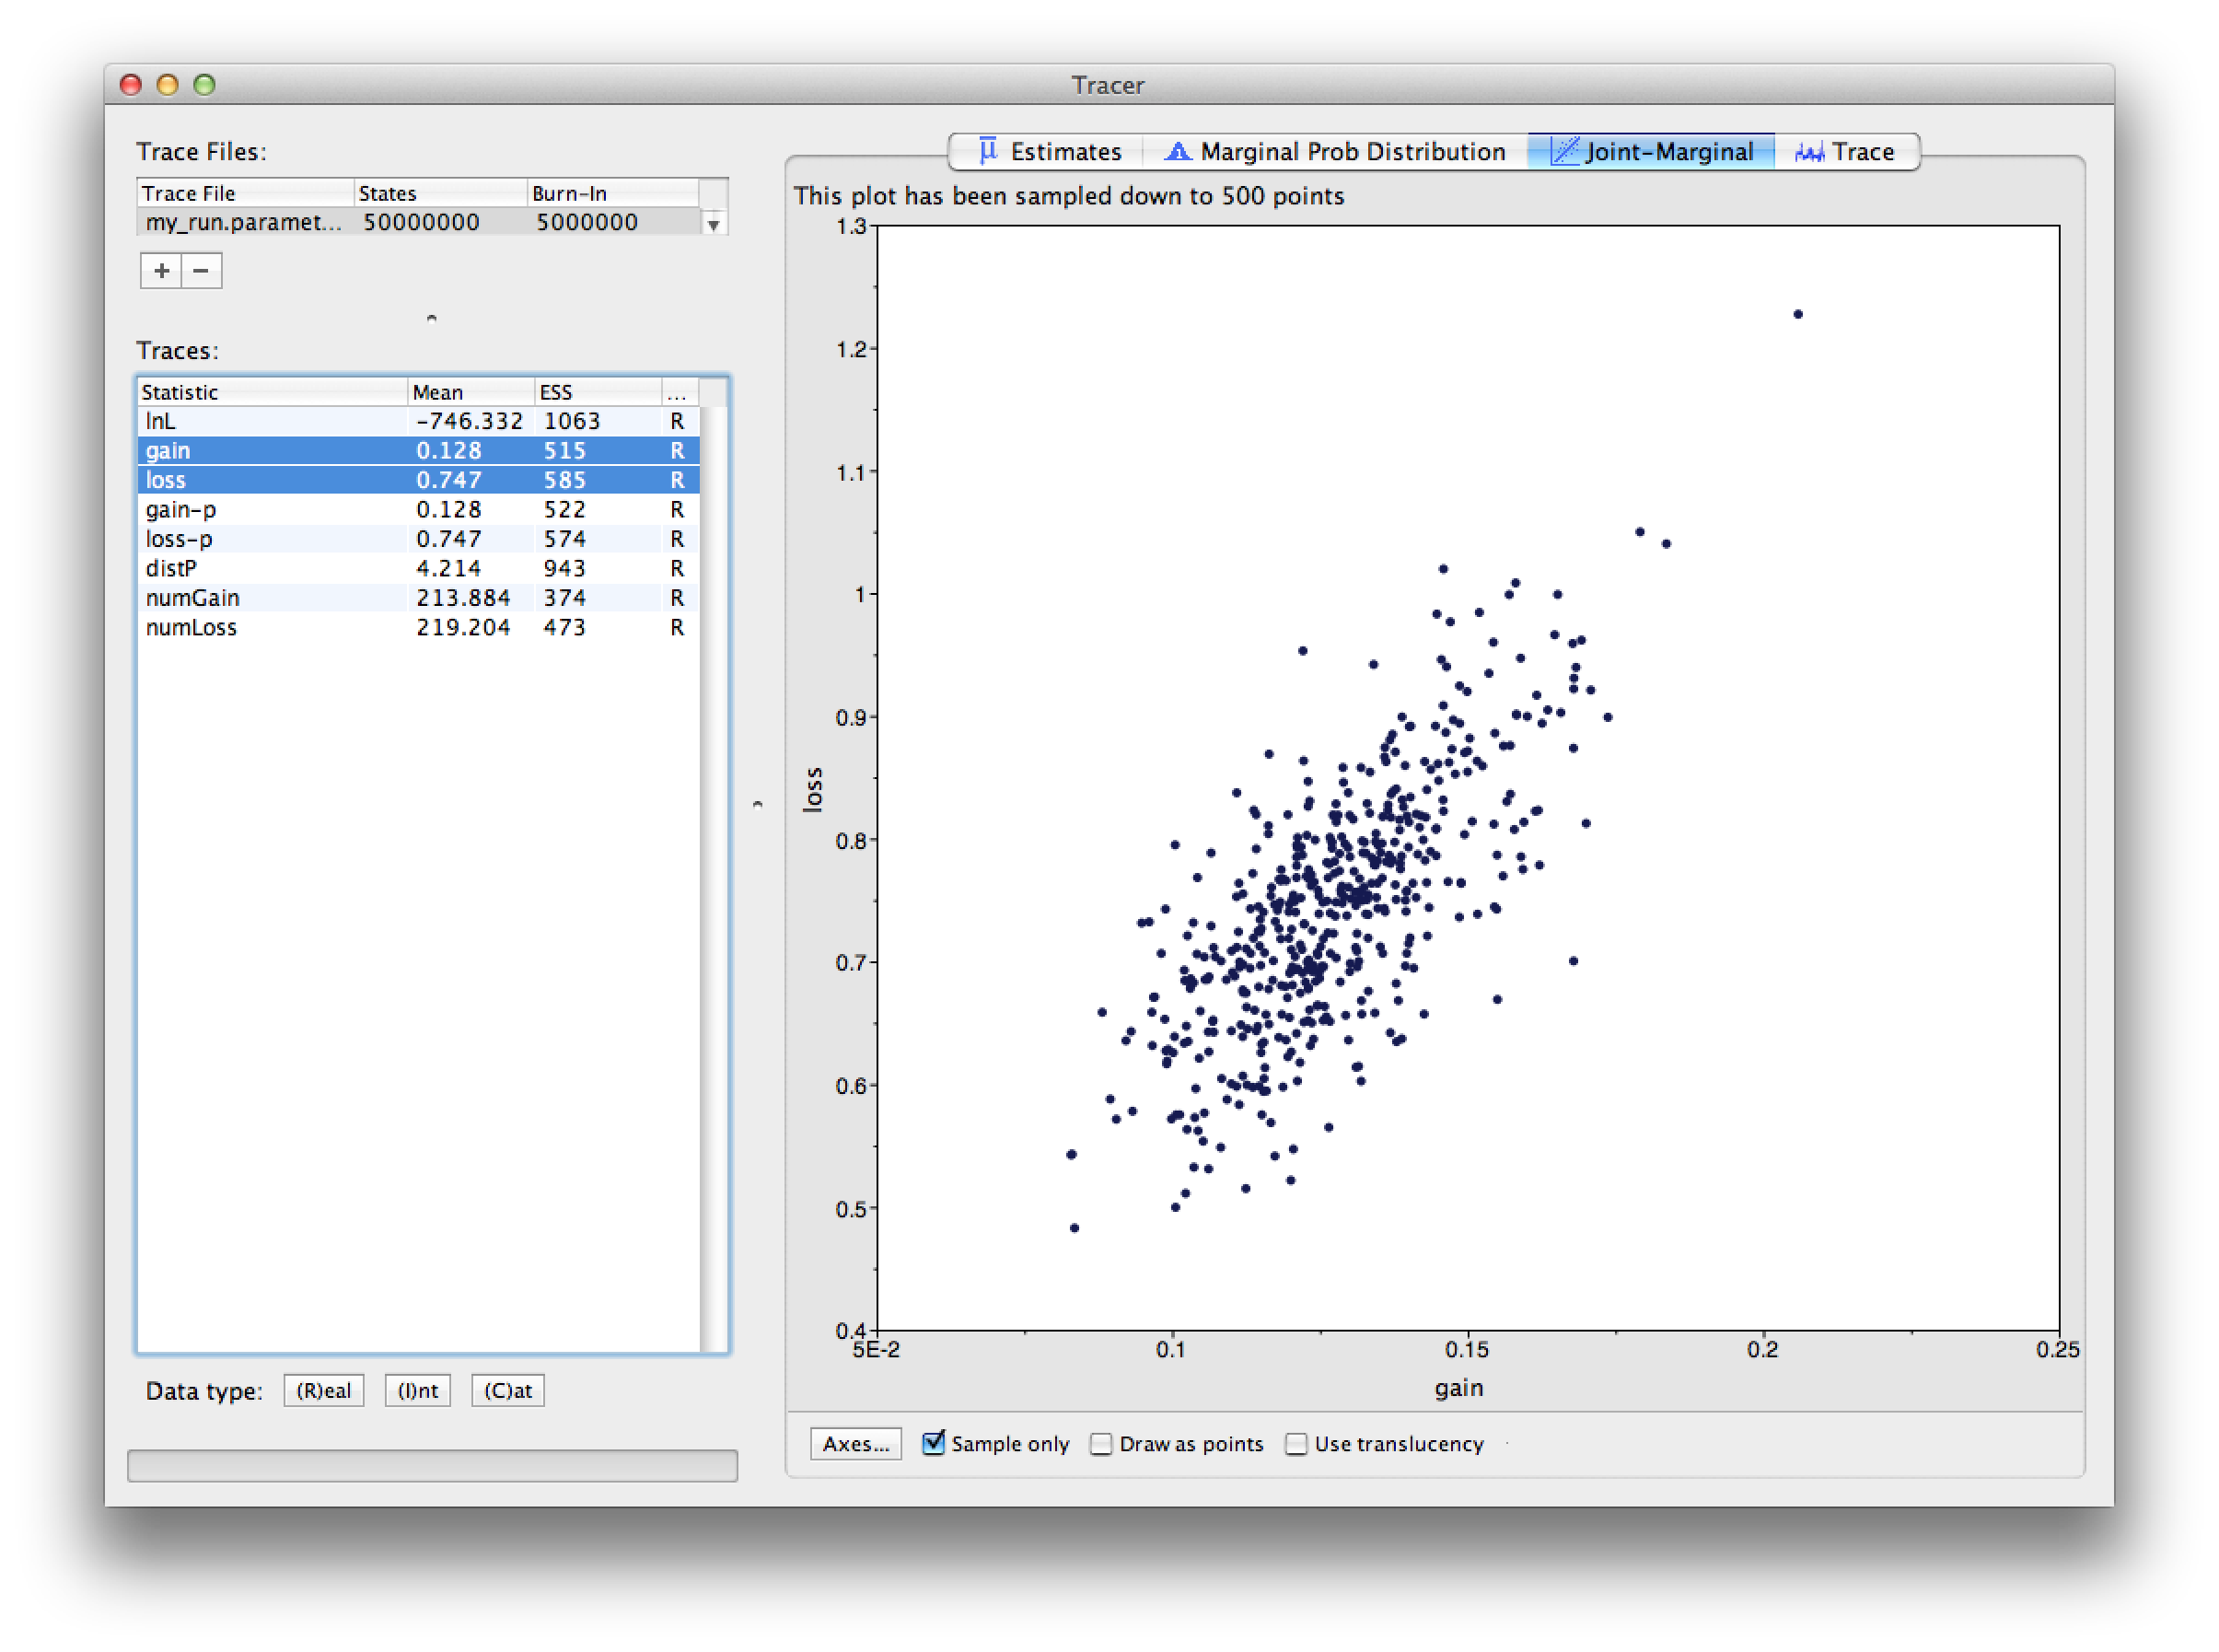
\includegraphics[width=2.5in]{figures/loss_gain}
\end{figure}

The Joint-Marginal of rate of area gain and loss parameters shows strong positive correlation.
This correlation arises partly because the proportion of occupied areas is greatly influenced by the ratio of rate of area gain to rate of area loss.
For example, when the rates of area gain and loss are equal, range sizes tend to equal half the total number of areas.

\noindent \\ \impmark Highlight the ``loss'' and ``numLoss'' parameters then click Joint-Marginal. Do the same for ``gain'' and ``numGain''. \\

\begin{figure}[H]
\centering
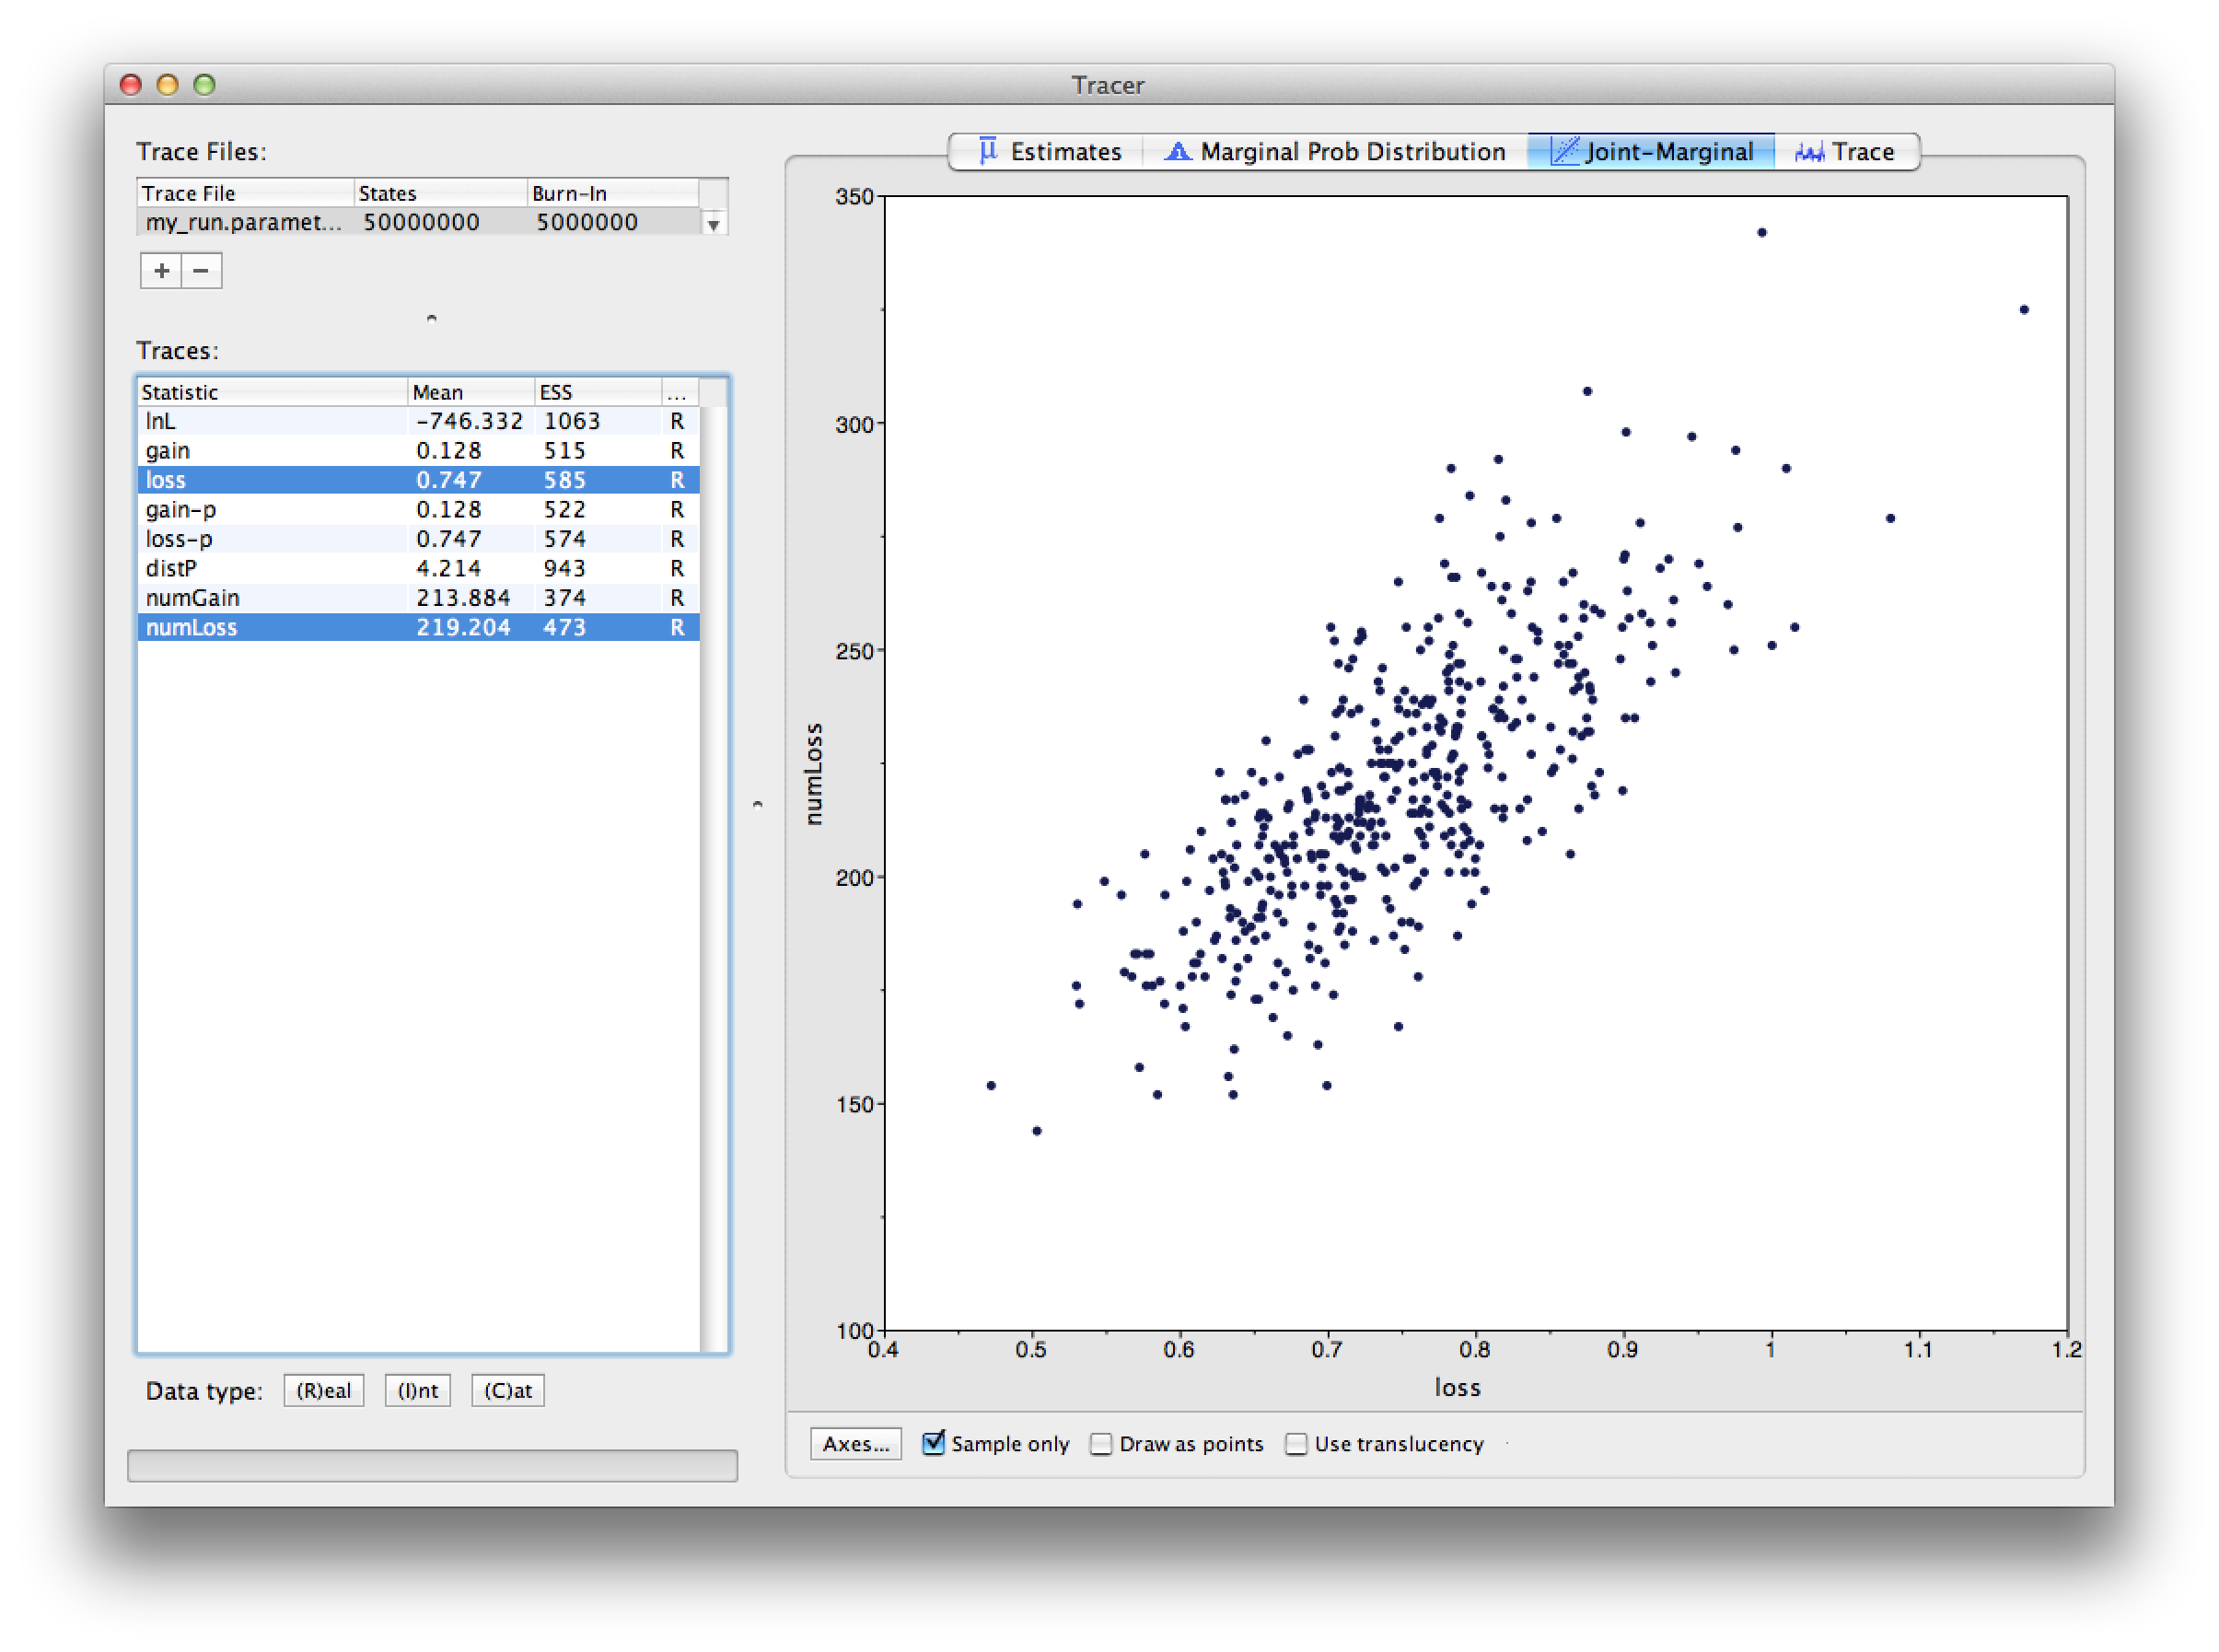
\includegraphics[width=2.5in]{figures/loss_numloss}
\end{figure}

Again, we see strong positive correlation.
This is reassuring, since we expect to see many sampled range gain and loss events when the corresponding rates are high.

\noindent \\ \impmark  Highlight the ``gain'' and ``distP'' parameters then click Joint-Marginal. Do the same for ``loss'' and ``distP''.\\

\begin{figure}[H]
\centering
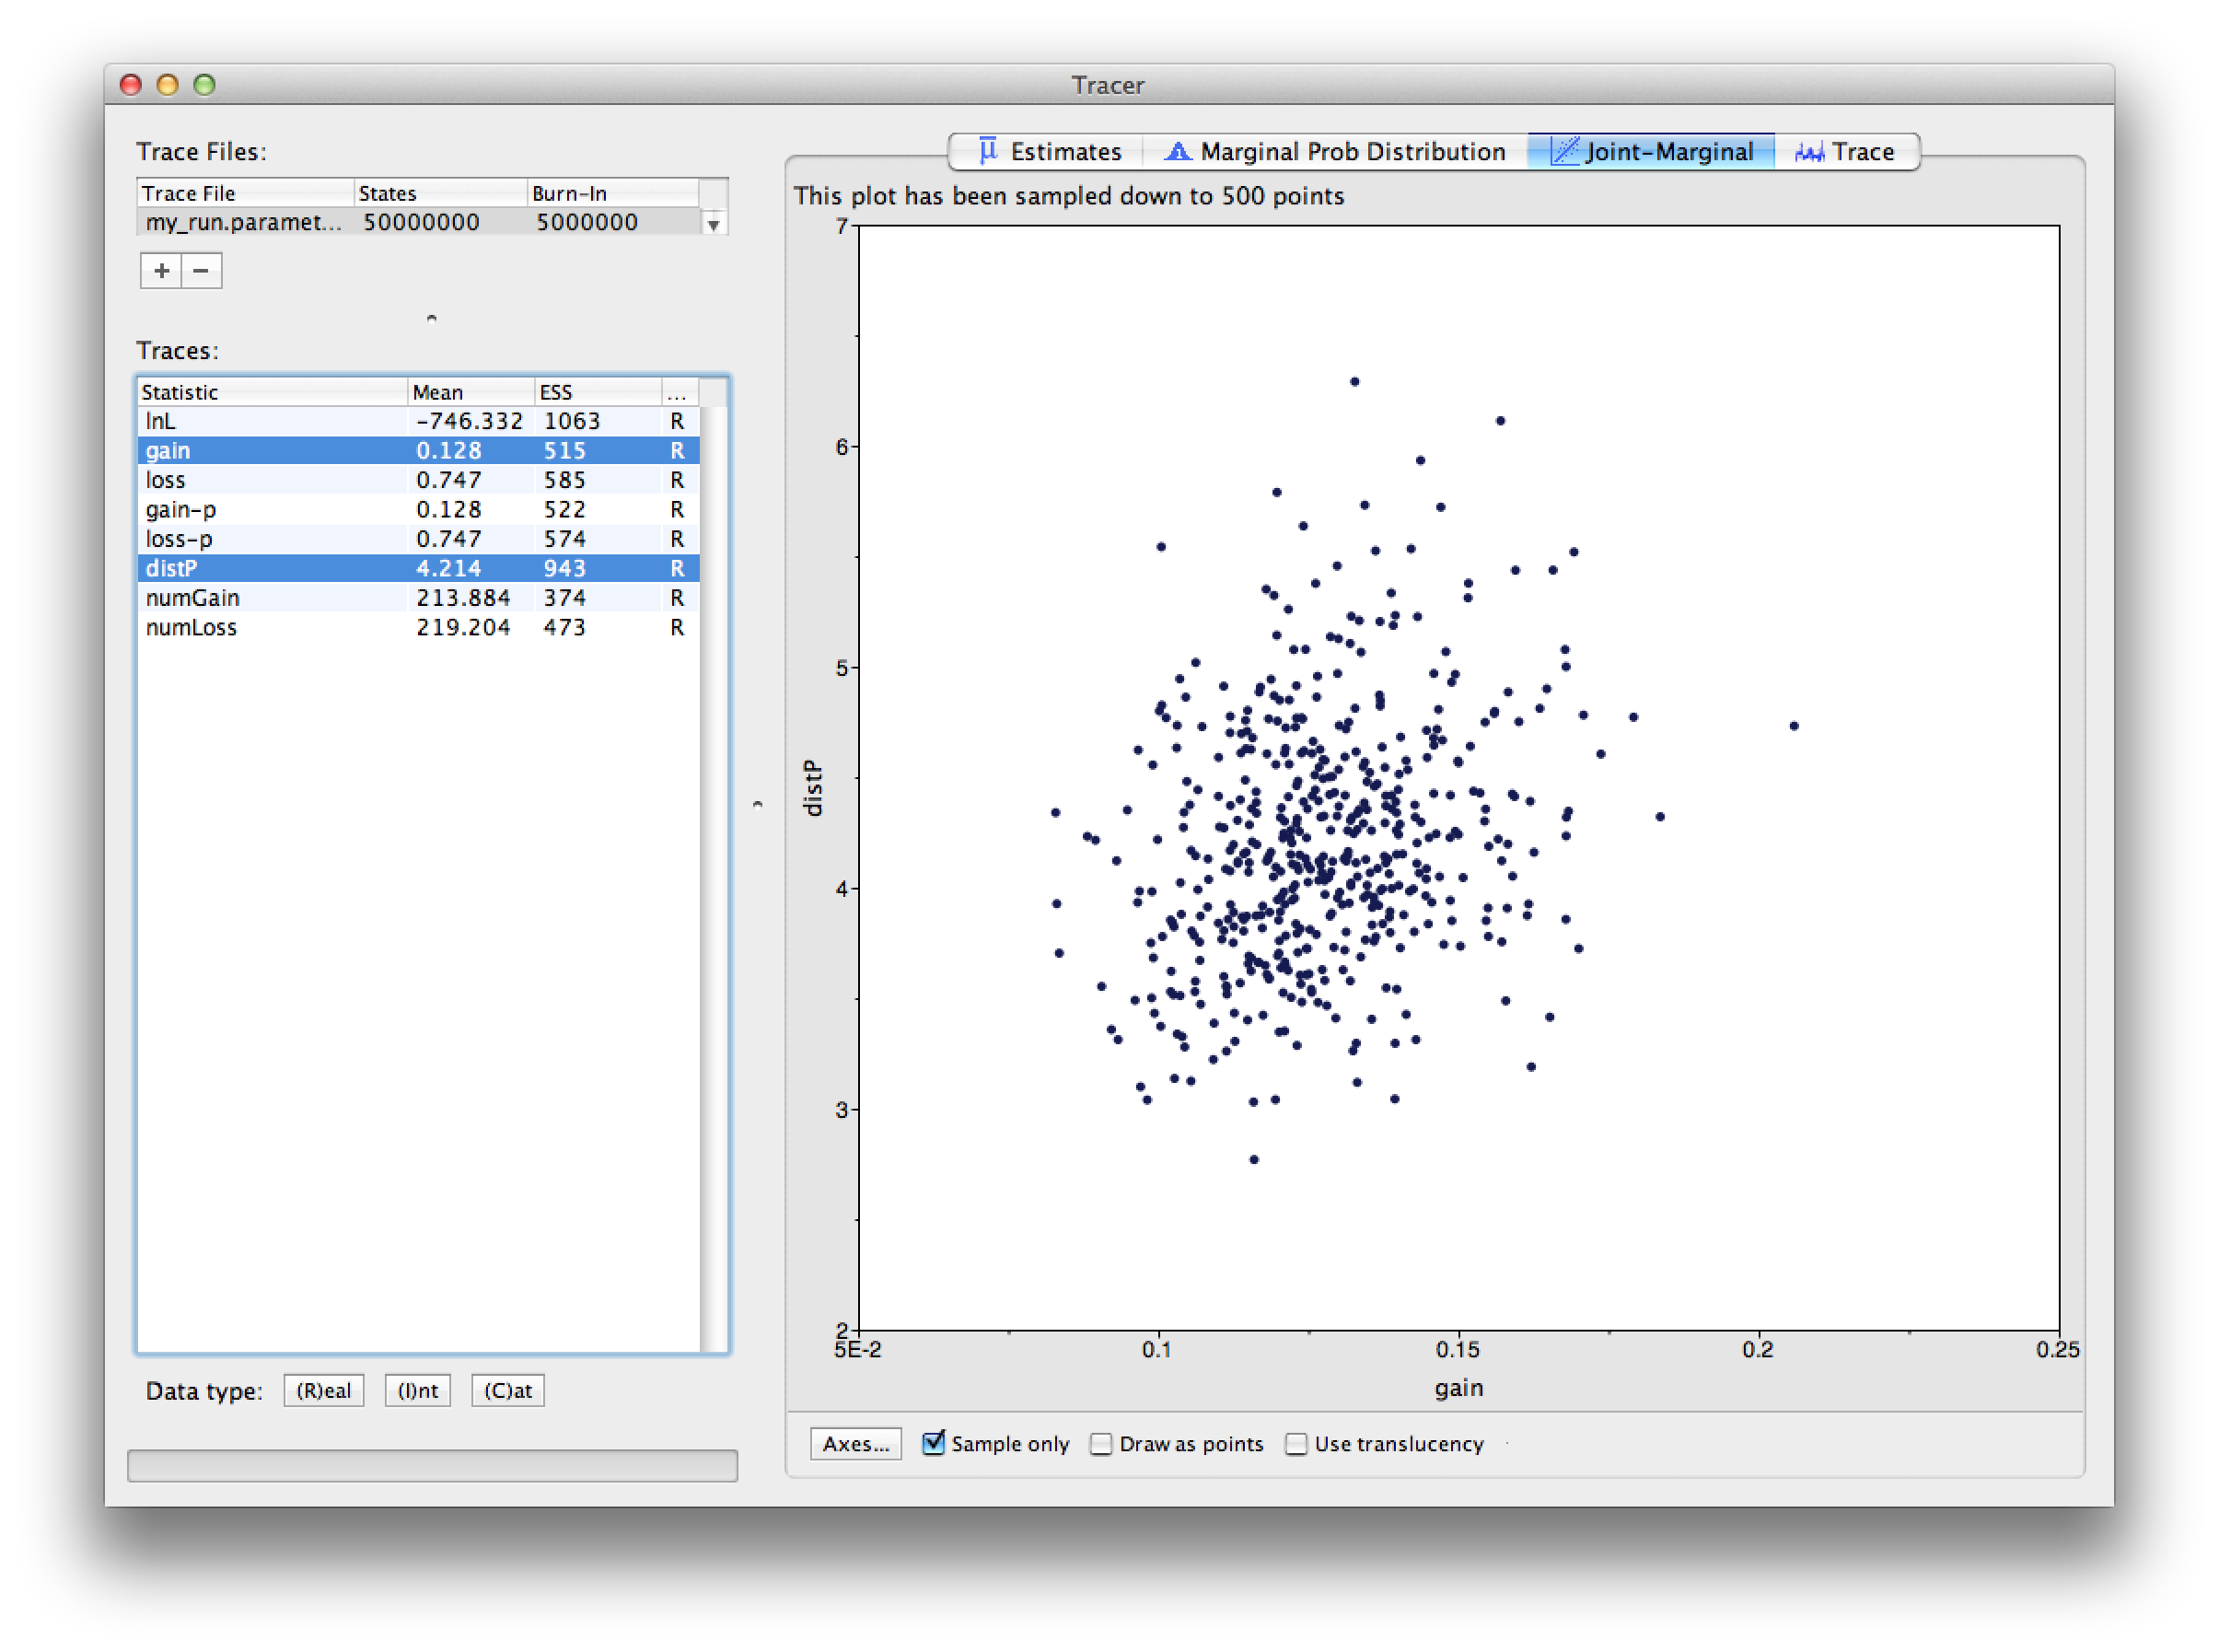
\includegraphics[width=2.5in]{figures/gain_distp}
\end{figure}

For the simulated data we don't see any strong correlation between either rate of loss or gain and the distance power parameter, but this is not always the case.
Large distance power parameters sometimes results in rates of area gain and loss being underestimated in value, resulting in a mild negative correlation.

\noindent \\ \impmark Highlight all parameters and click Estimates.

\begin{figure}[H]
\centering
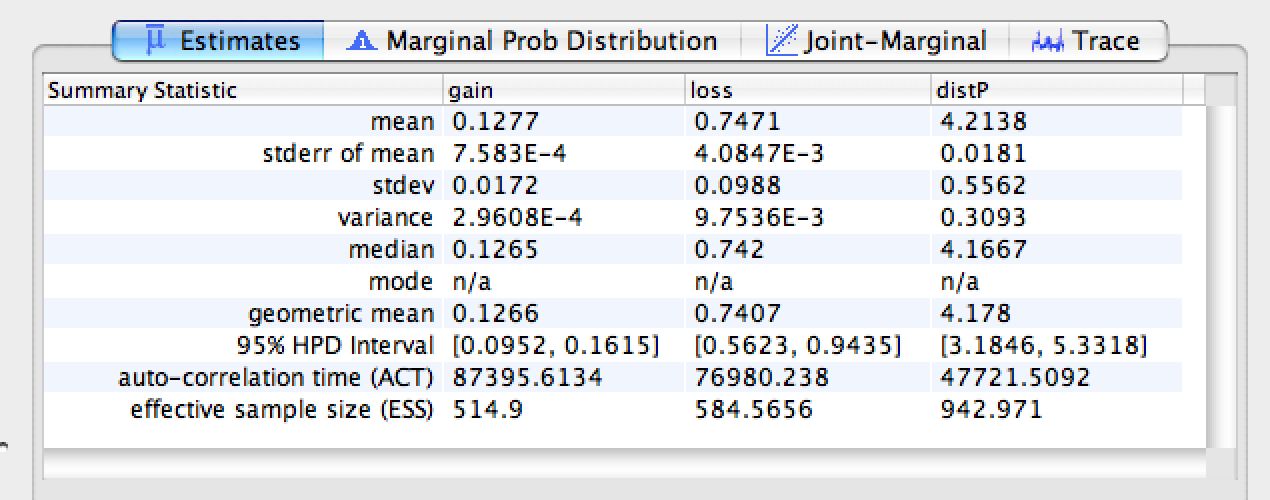
\includegraphics[width=2.5in]{figures/hpd}
\end{figure}

This gives you a handy selection of summary statistics.
Of course we typically don't know the true parameter values, but we should be reassured to learn the true parameter values for gain, loss, and distP (0.1, 0.7, and 4.0, respectively) reside within their corresponding 95\% HPD Intervals.
It's also interesting to note that the distance power parameter has a much wider interval that the rate parameters, suggesting there is less information in the data for this parameter.

%The Gelman-Rubin convergence diagnostic tests whether two MCMC analyses converged to the same distribution (e.g. the posterior).
%It does this by computing potential scale reduction factors (PSRFs) for all parameters, which compares the within-chain parameter variance to the between-chain parameter variance.
%There's no hard rule, but PSRF values close to 1.0 show convergence while PSRF values greater than 1.1 raise concern.
%Below, we can quickly compute the PSRFs for \texttt{my\_run.parameters.txt} and \texttt{my\_other\_run.parameters.txt} using the R package, coda.
%
%\noindent \\ \impmark Open the R console and enter the following commands.
%\begin{framed}
%\begin{lstlisting}
%> install.packages('coda')
%...
%> library('coda')
%> run1 = mcmc(read.table('my_run.parameters.txt',header=T))
%> run2 = mcmc(read.table('my_other_run.parameters.txt',header=T))
%> gelman.diag(mcmc.list(run1,run2))
%>
%Potential scale reduction factors:
%
%        Point est. Upper C.I.
%n              NaN        NaN
%lnL           1.00       1.00
%gain          1.01       1.01
%loss          1.00       1.01
%gain.p        1.00       1.01
%loss.p        1.00       1.01
%distP         1.00       1.00
%numGain       1.01       1.02
%numLoss       1.00       1.01
%
%Multivariate psrf
%
%1
%\end{listing}
%\end{framed}

\subsection{Sampled range histories (\texttt{my\_run.area\_states.txt})}

This file reports the stochastically mapped range histories sampled every \texttt{historySampleFrequency} iterations.
From this we can compute the {\it marginal} posterior probability of any given area being occupied simply by finding the frequency the area was marked present (1), which we'll call the {\it marginal area posterior probability}.
You may be interested in not only the marginal posterior of area occupancy, but the marginal posterior of the joint distribution of areas, which we'll call the {\it marginal range posterior probability}.
For example, say your range contains 4 areas, and taxon A is present only in areas 1 and 2 for half of all MCMC samples and only present in areas 3 and 4 for the remaining half.
The marginal area posterior range would report a 0.5 probability of any given area being occupied.
The marginal range posterior would give you richer information, that the range was either composed of areas 1 and 2 or of 3 and 4, but never 1 and 3, 1 and 4, 2 and 3, or 2 and 4.

Here we will use Python to report the marginal range probability for the range belonging to the most recent common ancestor (MRCA) shared by the species named \texttt{t1} and \texttt{t2} ordered by their posterior probabilities. We'll call this node MRCA(t1,t5).

\noindent \\ \impmark Change directories to \texttt{examples}.

\begin{framed}
\begin{lstlisting}
> cd examples
\end{lstlisting}
\end{framed}

\noindent \\ \impmark Open the Python console and enter the following commands.

\begin{framed}
\begin{lstlisting}
>>> from pp_range import *
>>> range_dict = make_range_dict('my_run.area_states.txt', fburn=0.25)
>>> area_coords = get_area_coords('my_geo.txt')
>>> idx_list = get_node_idx_list('my_run.area_states.txt')
>>> node_key = get_node_key('my_tree.txt', 't1', 't5', idx_list)
>>> best_ranges = get_best_ranges(range_dict, node_key)
>>> prob_area_pairs = make_posterior_area_pairs(range_dict, node_key)
>>> best_area_pairs = get_best_area_pairs(prob_area_pairs)
>>> best_areas = get_best_area_pairs(prob_area_pairs, show_marginal=True)
\end{lstlisting}
\end{framed}

\noindent \\ \impmark To list the five most probable ranges for MRCA(t1,t5), type
\begin{framed}
\begin{lstlisting}
>>> best_ranges[0:5]
[('000000000000000000000000001111000', 0.022660623833644103),
 ('000000000000000000000000001011000', 0.01759530791788836),
 ('000000000000000000000000011111000', 0.01652892561983452),
 ('000000000000000000000000011011000', 0.0146627565982403),
 ('000000000000000000010000001111000', 0.01226339642761916)]

>>> sum([p[1] for p in best_ranges[0:5]])
0.08371101039722645
\end{lstlisting}
\end{framed}

The second column gives the probability of the entire MRCA(t1,t5) range shown in the first column.
There's a fair deal of uncertainty the MRCA(t1,t5) range reconstruction, since these best five ranges only account for about 0.08 of the probability.

\noindent \\ \impmark To list the five most probable area co-occurrences in the MRCA(t1,t5) range, type
\begin{framed}
\begin{lstlisting}
>>> best_area_pairs[0:5]
[((26, 29), 0.60650493201812505),
 ((26, 28), 0.57717941882164425),
 ((28, 29), 0.54385497200746136),
 ((26, 27), 0.42282058117834981),
 ((27, 28), 0.41242335377232475)]
 
>>> best_areas[0:5]
[((26, 26), 0.78459077579311998),
 ((29, 29), 0.77179418821647394),
 ((28, 28), 0.74193548387096575),
 ((26, 29), 0.60650493201812505),
 ((26, 28), 0.57717941882164425)]

\end{lstlisting}
\end{framed}

Note the values in \texttt{best\_areas} are the marginal area probabilities.
These correspond to the diagonal entries in the heatmap below and to the values in \texttt{my\_run.area\_probs.txt} and \texttt{my\_run.nhx}.

\noindent \\ \impmark To visualize these probabilities as a heatmap, type
\begin{framed}
\begin{lstlisting}
>>> title_str = 'Prob(areas i,j co-occur in MRCA(t1,t5) range)'
>>> plot_posterior_area_pair(prob_area_pairs, title_str)
\end{lstlisting}
\end{framed}

\begin{figure}[H]
\centering
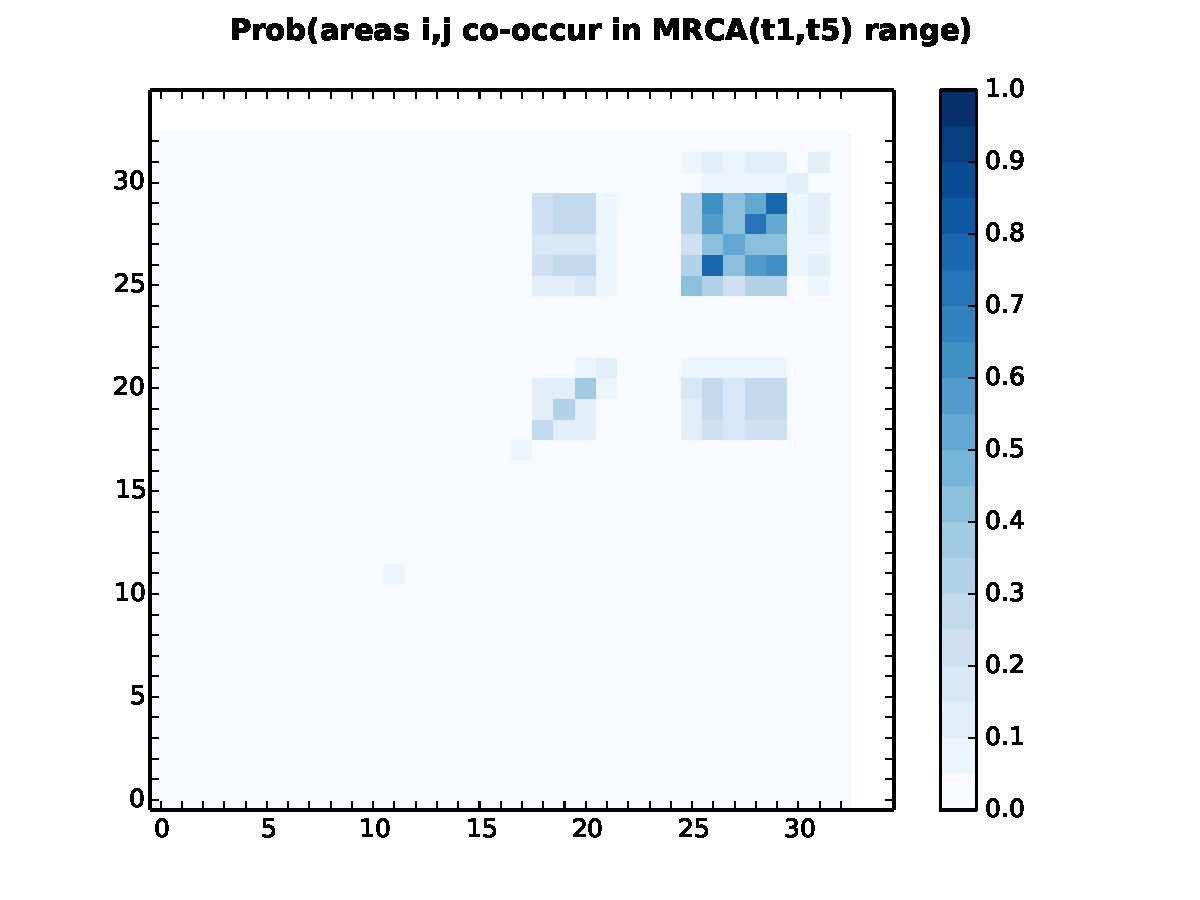
\includegraphics[width=4in]{figures/range_area_pair_pp}
\end{figure}

As indicated from the list produced by \texttt{get\_best\_area\_pairs()}, we see the inference gives moderate support for areas 26, 28, and 29 being co-occupied by MRCA(t1,t5).
Referring to \texttt{my\_geo.txt}, we see these areas are geographically close and located in south-eastern Australia.
You can also retrieve the coordinates through the \texttt{area\_coords} dictionary.

\noindent \\ \impmark To query the geographical coordinates for an area, type
\begin{framed}
\begin{lstlisting}
>>> area_coords[26]
{'lat': -32.5, 'lon': 137.5}

>>> area_coords[28]
{'lat': -32.5, 'lon': 147.5}

>>> area_coords[29]
{'lat': -32.5, 'lon': 152.5}
\end{lstlisting}
\end{framed}

\subsection{Posterior probabilities of range histories (\texttt{my\_run.area\_probs.txt})}

Each row of this tab-delimited file contains information about that node's range.
The rows are ordered in postorder traversal (aka pruningwise).
The first column gives the taxon name.
The remaining columns correspond to areas, maintaining the same order as all other files (e.g. the second column is the first area, the $n$th column is the ($n-1$)th area).
These entries report the marginal area probability of the taxon (row) occupying the area (column).
These probabilities are computed the frequency that the area was marked present from the data contained in \texttt{my\_run.area\_probs.txt}, a quantity that cannot be computed until the MCMC analysis completes.
Because MCMC does not accurately sample from posterior during burn-in, some number of initial cycles are discarded as specified by the \texttt{probBurnIn} flag.

\subsection{New Hampshire extended format file (\texttt{my\_run.nhx})}

This file summarizes the input and output from a BayArea analysis using NEXUS format containing a New Hampshire eXtended (NHX) tree string.
NHX allows you to annotate nodes in a Newick string with meta-information, which BayArea uses to report the probabilities in the \texttt{my\_run.area\_probs.txt} file.
The \texttt{geo} block gives the geographical latitudes and longitudes for the areas in the order they are reported as probabilities.
Like the \texttt{my\_run.area\_probs.txt} file, this file is not written until the analysis is complete.
This annotation is used for the two visualization programs covered in the next section, Phylowood and BayArea-Fig.
The anatomy of the Phylowood and BayArea-Fig settings blocks will also be explained there.

\section{Visualization}

Here we'll explore two options for visualizing ancestral range reconstructions.
I'll walk you through some of the basic functionality, but feel free to play around as you like.

\subsection{Phylowood}

Phylowood generates interactive animations to explore biogeographic reconstructions.

\noindent \\ \impmark Open \texttt{http://mlandis.github.io/phylowood}.

\noindent \\ \impmark Drag and drop \texttt{my\_run.nhx} into the text field.

\begin{figure}[H]
\centering
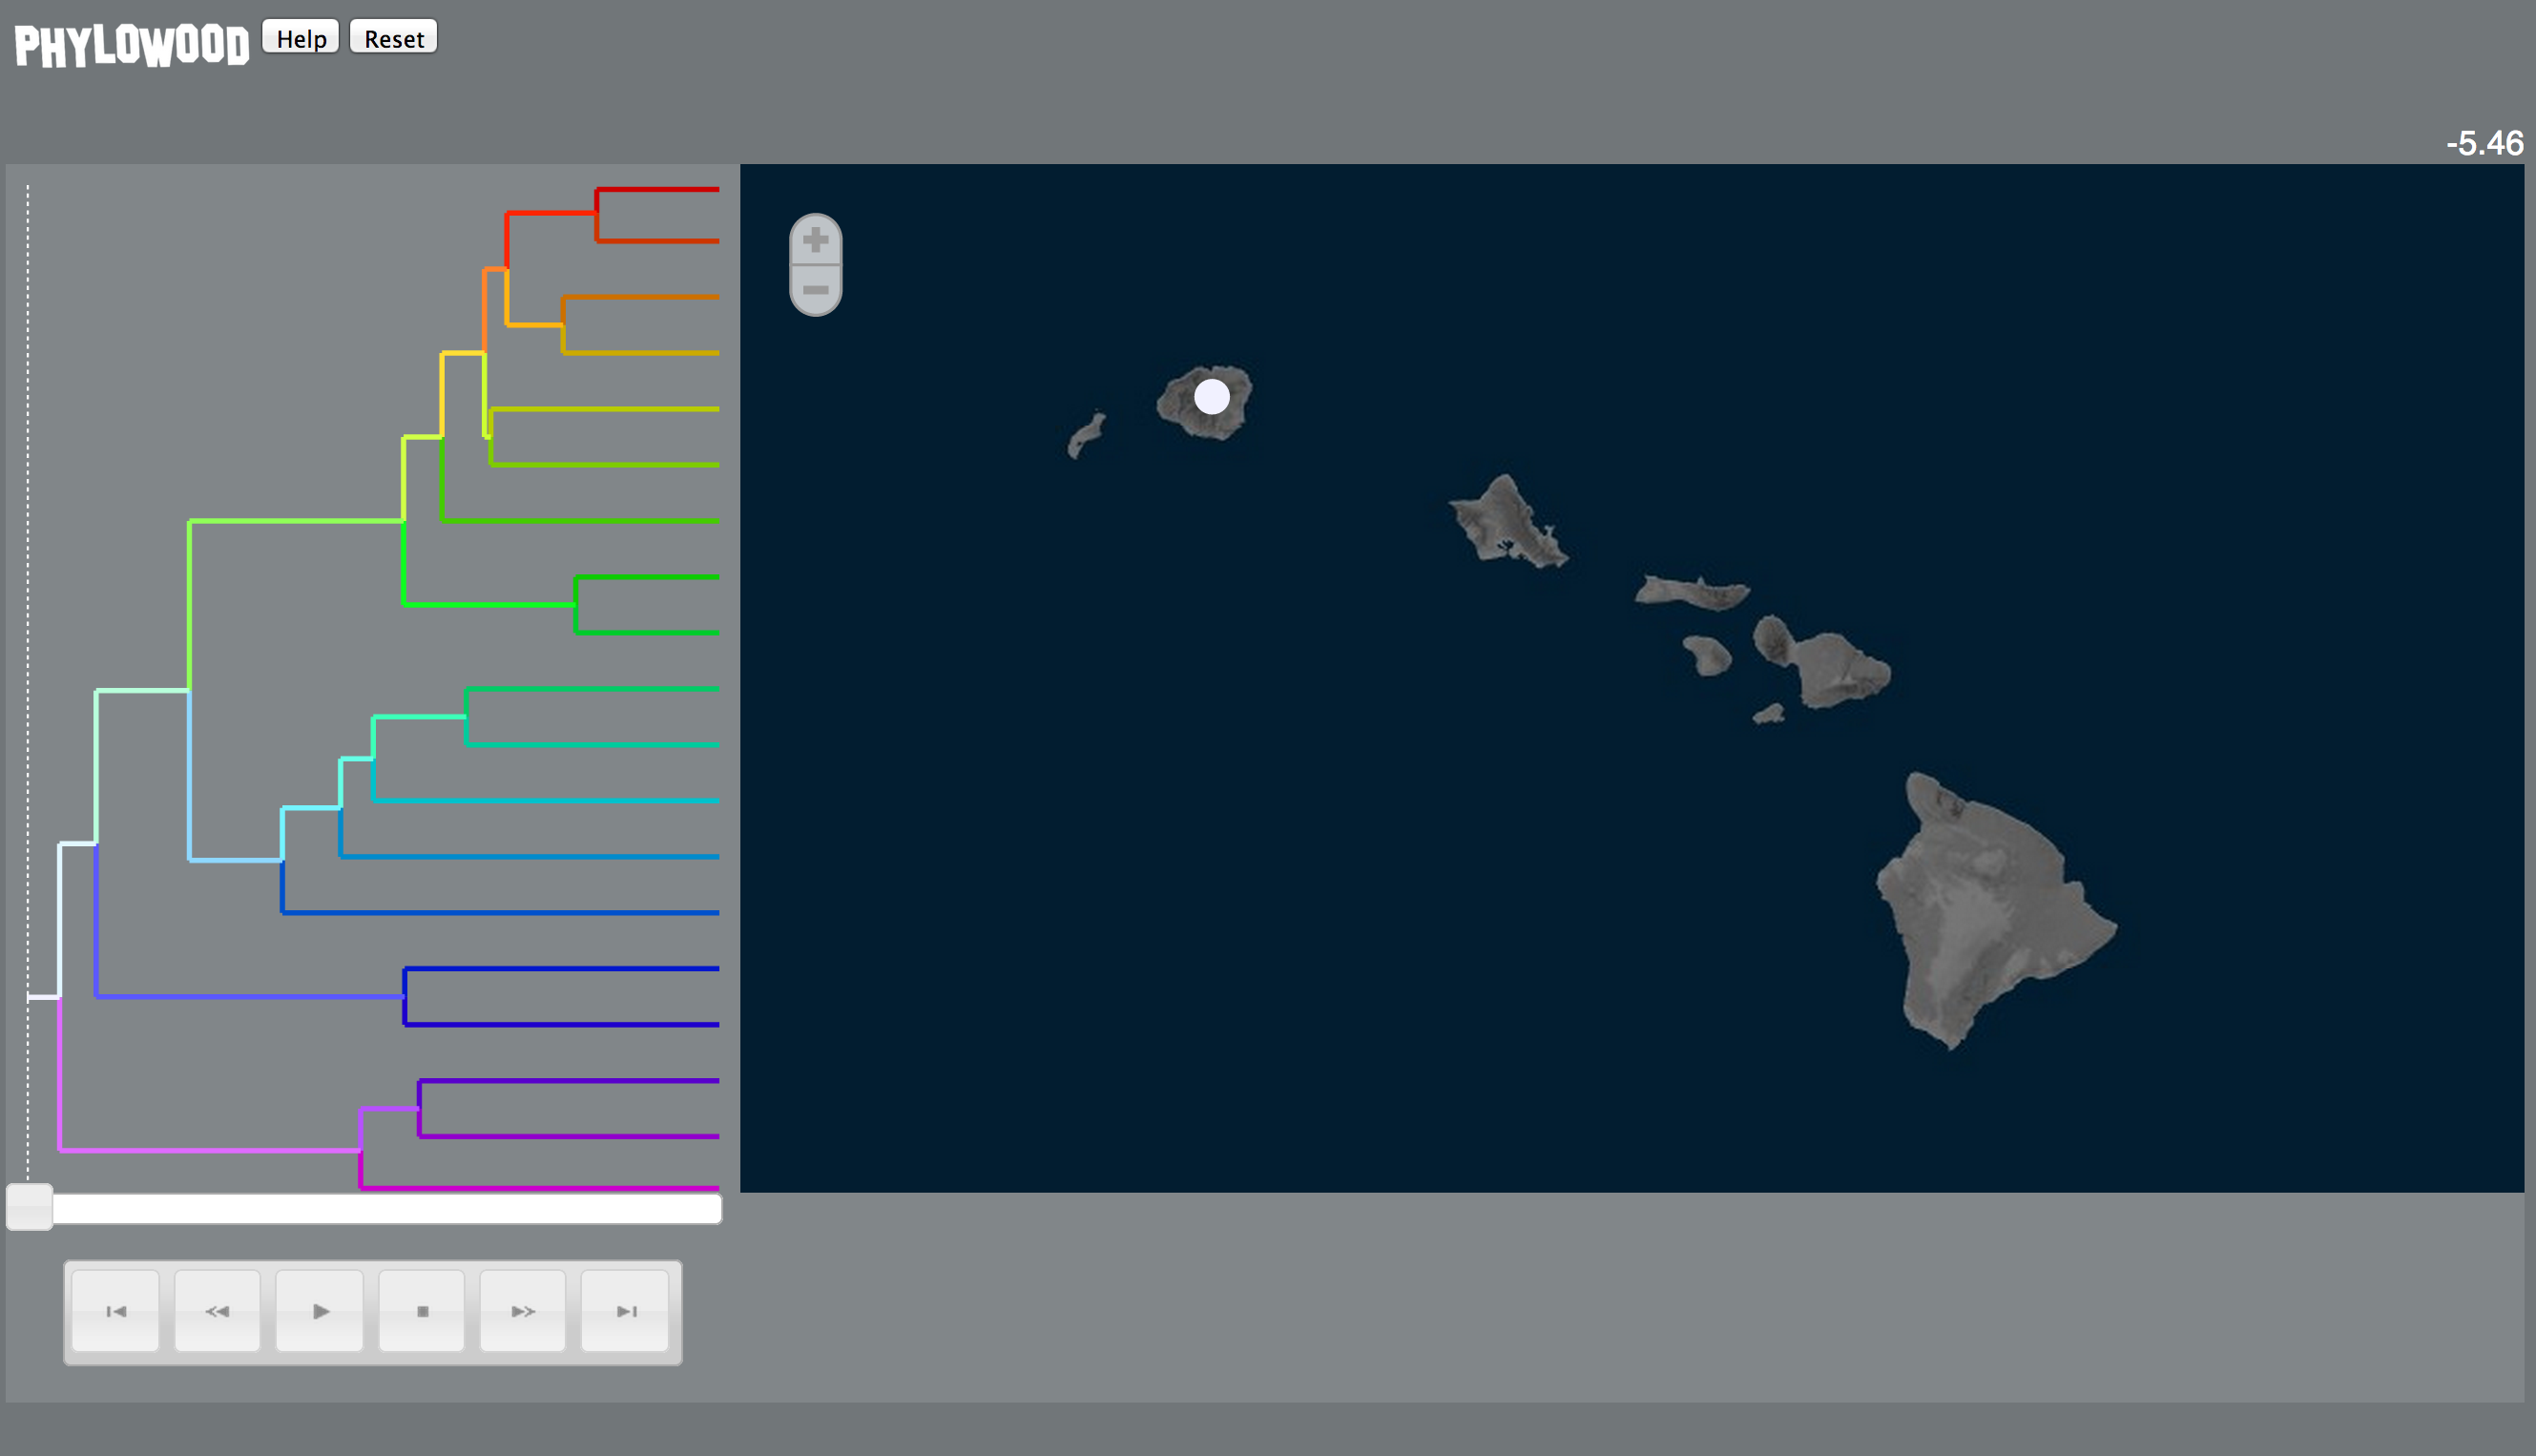
\includegraphics[width=4in]{figures/phw_mrca}
\end{figure}

\noindent \\ \impmark Click the Play button to view the animation. \\

There are three control panels to help you filter data: the media panel, the map panel, and the phylogeny panel.
The media buttons correspond to Beginning, Slow/Rewind, Play, Stop, Fast Forward, Ending (from left to right).
The animation will play the timeframe corresponding to the slider.

\noindent \\ \impmark Drag the slider to the time marked ``-1.1'' in the upper right corner.

\begin{figure}[H]
\centering
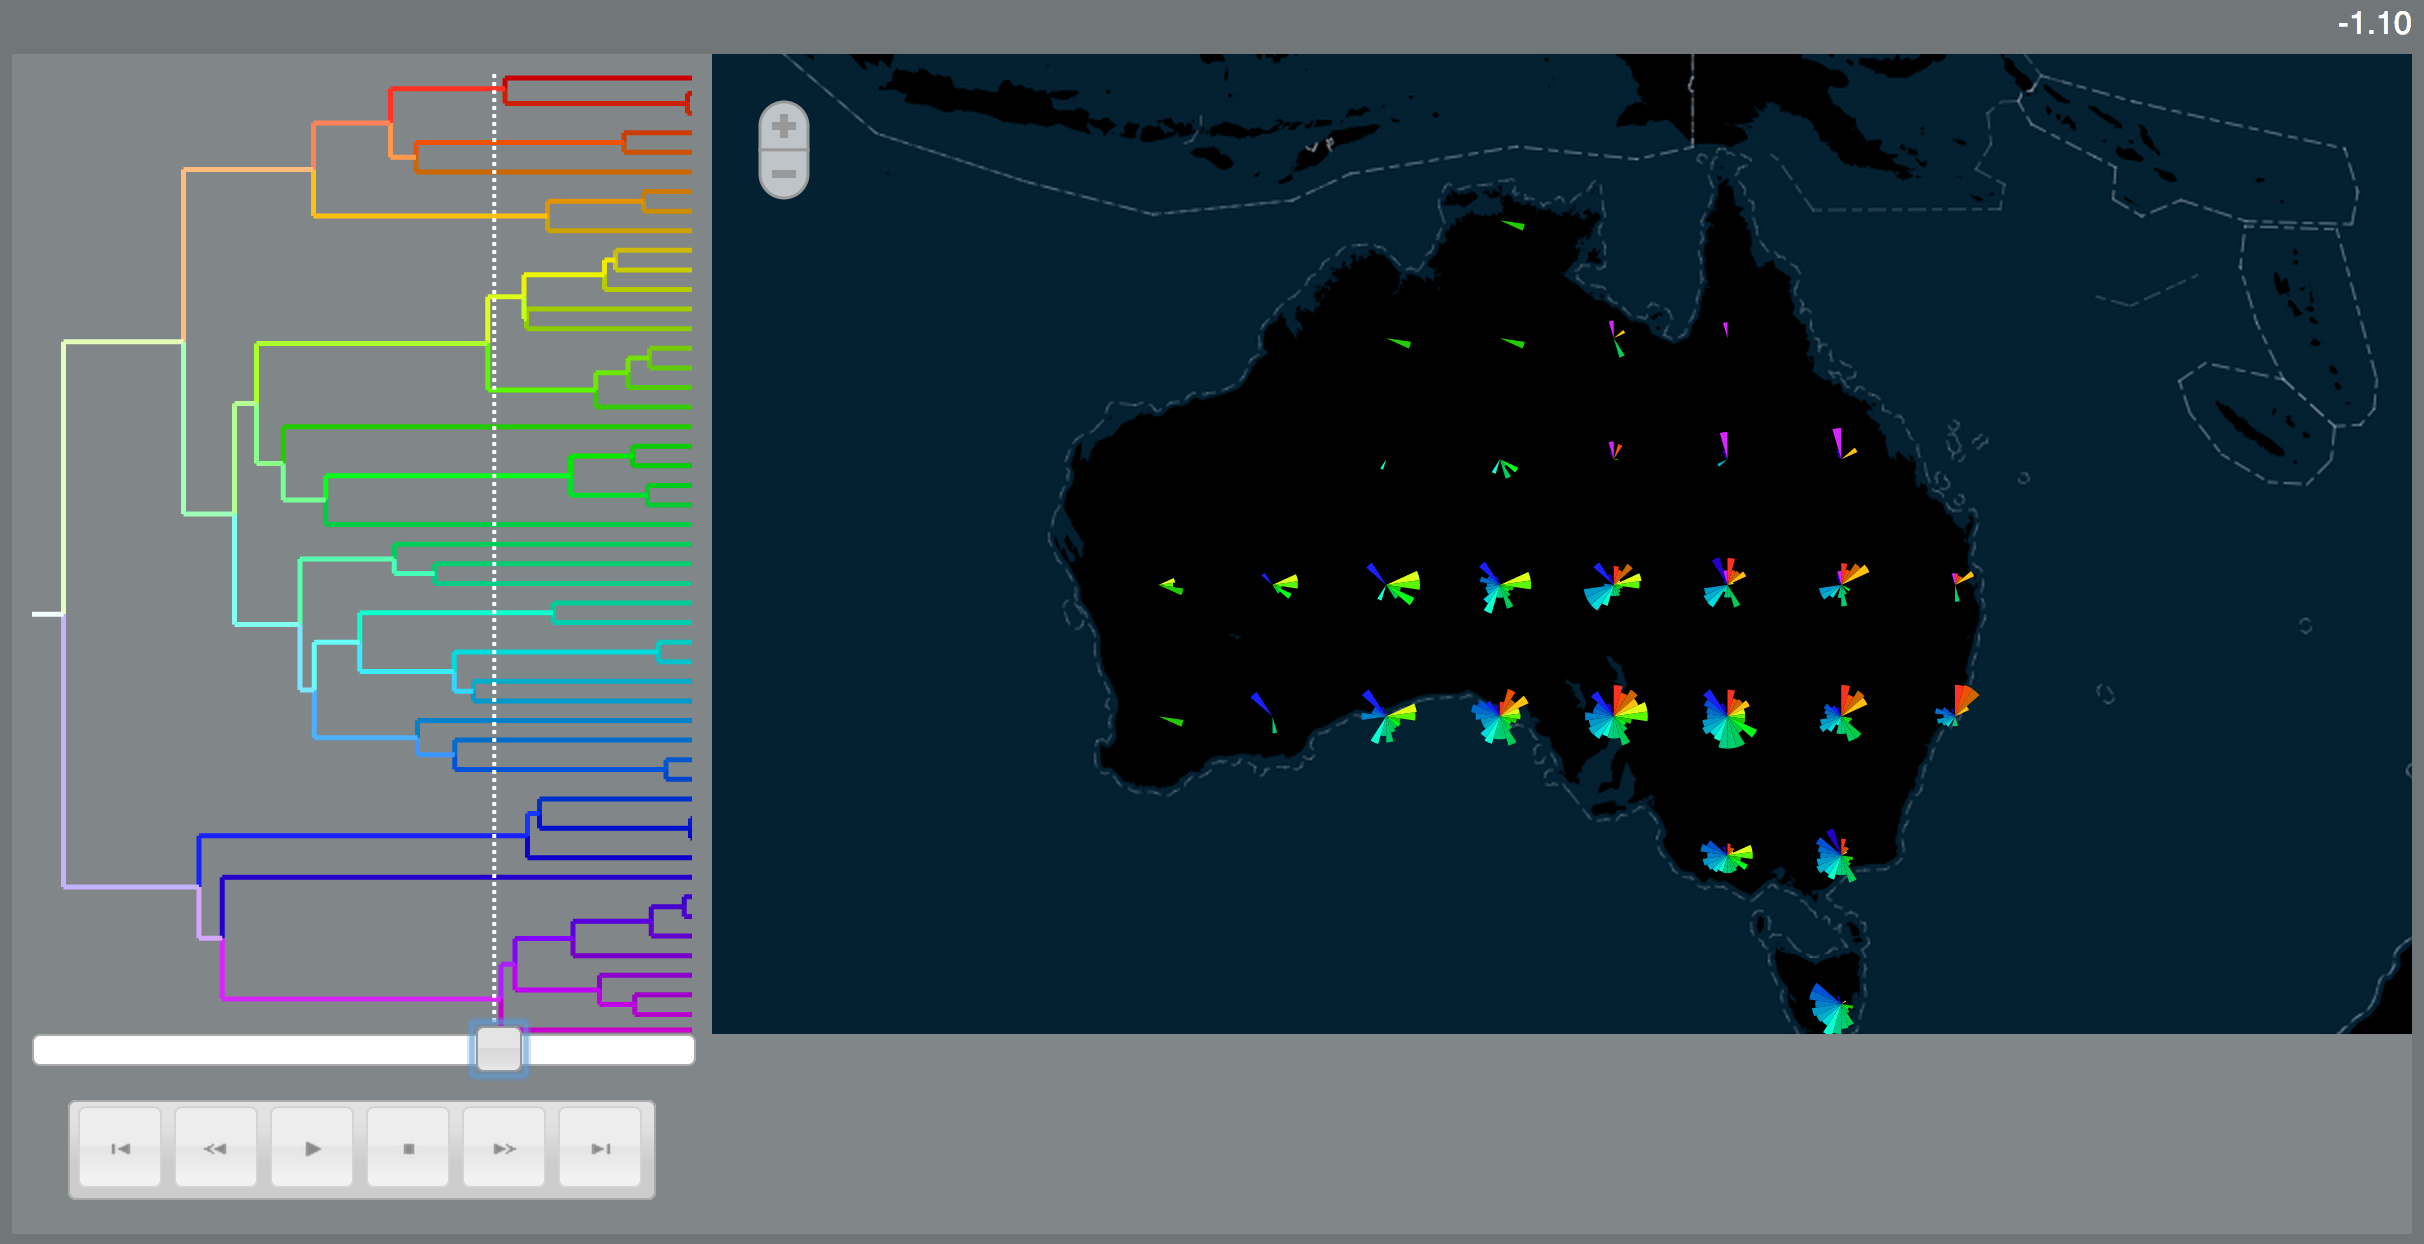
\includegraphics[width=4in]{figures/phw_1_1ma}
\end{figure}

\noindent \\ \impmark Pan and zoom around the map.\\

Marker colors correspond to the phylogenetic lineages in the phylogeny panel.
Markers are split into slices and (loosely) sorted phylogenetically, so nearby slices are generally closely related.
At divergence events, a marker's radius is proportional to the marginal posterior probability the node was present in the area at that time.
Between divergence events, marker's radius is simply an interpolation of the values at the two endpoints.

\noindent \\ \impmark Mouseover an area to learn which lineage it belongs to and its presence probability. \\

Since it's difficult to see how specific clades evolve with so many taxa, Phylowood offers two ways to filter taxa from the animation.
We call the set of a lineage, all its ancestral lineages towards the root, and all descendant lineages a phylogenetic heritage.
The root's heritage is the entire clade.
A leaf node's heritage is a path from the tip to the root.

\noindent \\ \impmark Mouseover a lineage to temporarily highlight the lineage's heritage. Remove the mouseover to remove the highlight effect. \\

The highlight effect is temporary and quickly allows you to single out lineages of interest during animation.
Phylowood also offers a masking effect that persists until an unmask command is issued.

\noindent \\ \impmark Double-click the white root branch to mask the root node's heritage (all lineages). Single click a lineage to unmask that lineage's heritage. \\

\begin{figure}[H]
\centering
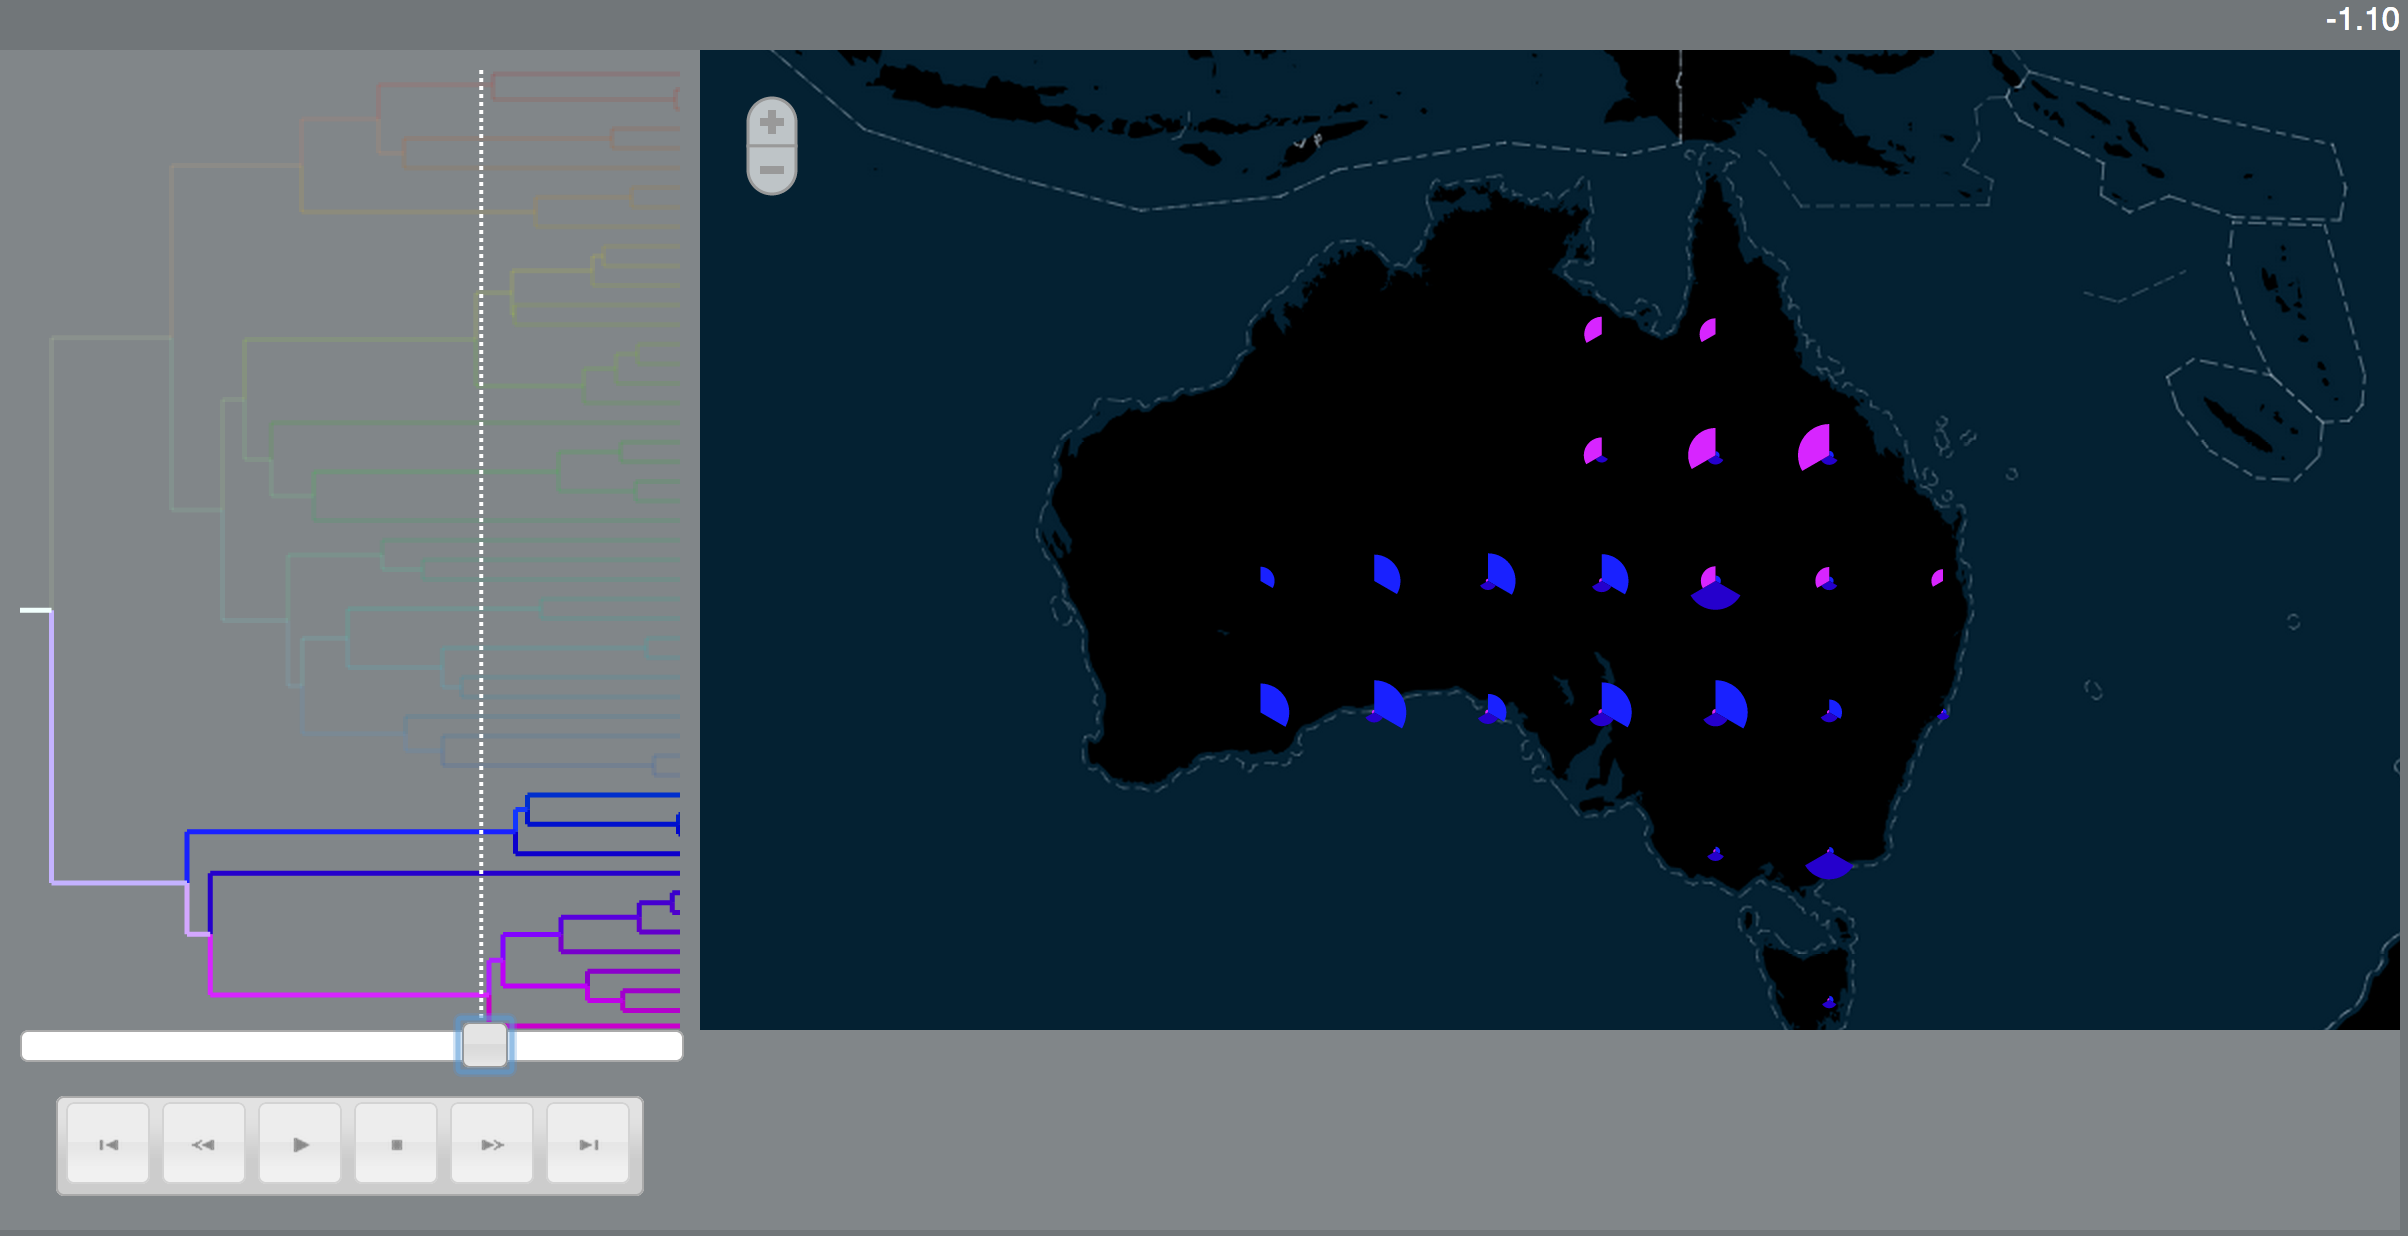
\includegraphics[width=4in]{figures/phw_mask}
\end{figure}

Now that the masking effects are in place, you're free to interact with other map components.
In addition, the area of marker sizes is only distributed among unmasked lineages.

\noindent \\ \impmark Visit \texttt{https://github.com/mlandis/phylowood/wiki} to learn more about Phylowood.


\subsection{BayArea-Fig}

BayArea-Fig is a simple Javascript utility to help generate ancestral range reconstruction figures for publications.
BayArea 1.0.2 does not automatically generate the NEXUS settings block for BayArea-Fig, so I added the following block to \texttt{my\_run.nhx}.

%\noindent \\ \impmark  Add the following code after the \texttt{\#NEXUS} header in \texttt{my\_run.nhx} and save the file.
\begin{framed}
\begin{lstlisting}
Begin bayarea-fig;
	mapheight 100
	mapwidth 150
	canvasheight 2000
	canvaswidth 2000
	minareaval 0.1
	areacolors blue red
	areatypes 0 1 0 0 0 1 1 0 0 0 0 1 1 1 0 0 0 0 1 1 1 1 0 0 0 0 1 1 1 1 1 1 1
	areanames West East
End;
\end{lstlisting}
\end{framed}

\noindent \\ \impmark  Open \texttt{http://mlandis.github.io/bayarea-fig} in a web browser.

\noindent \\ \impmark  Drag and drop \texttt{my\_run.nhx} into the text field. \\

\begin{figure}[H]
\centering
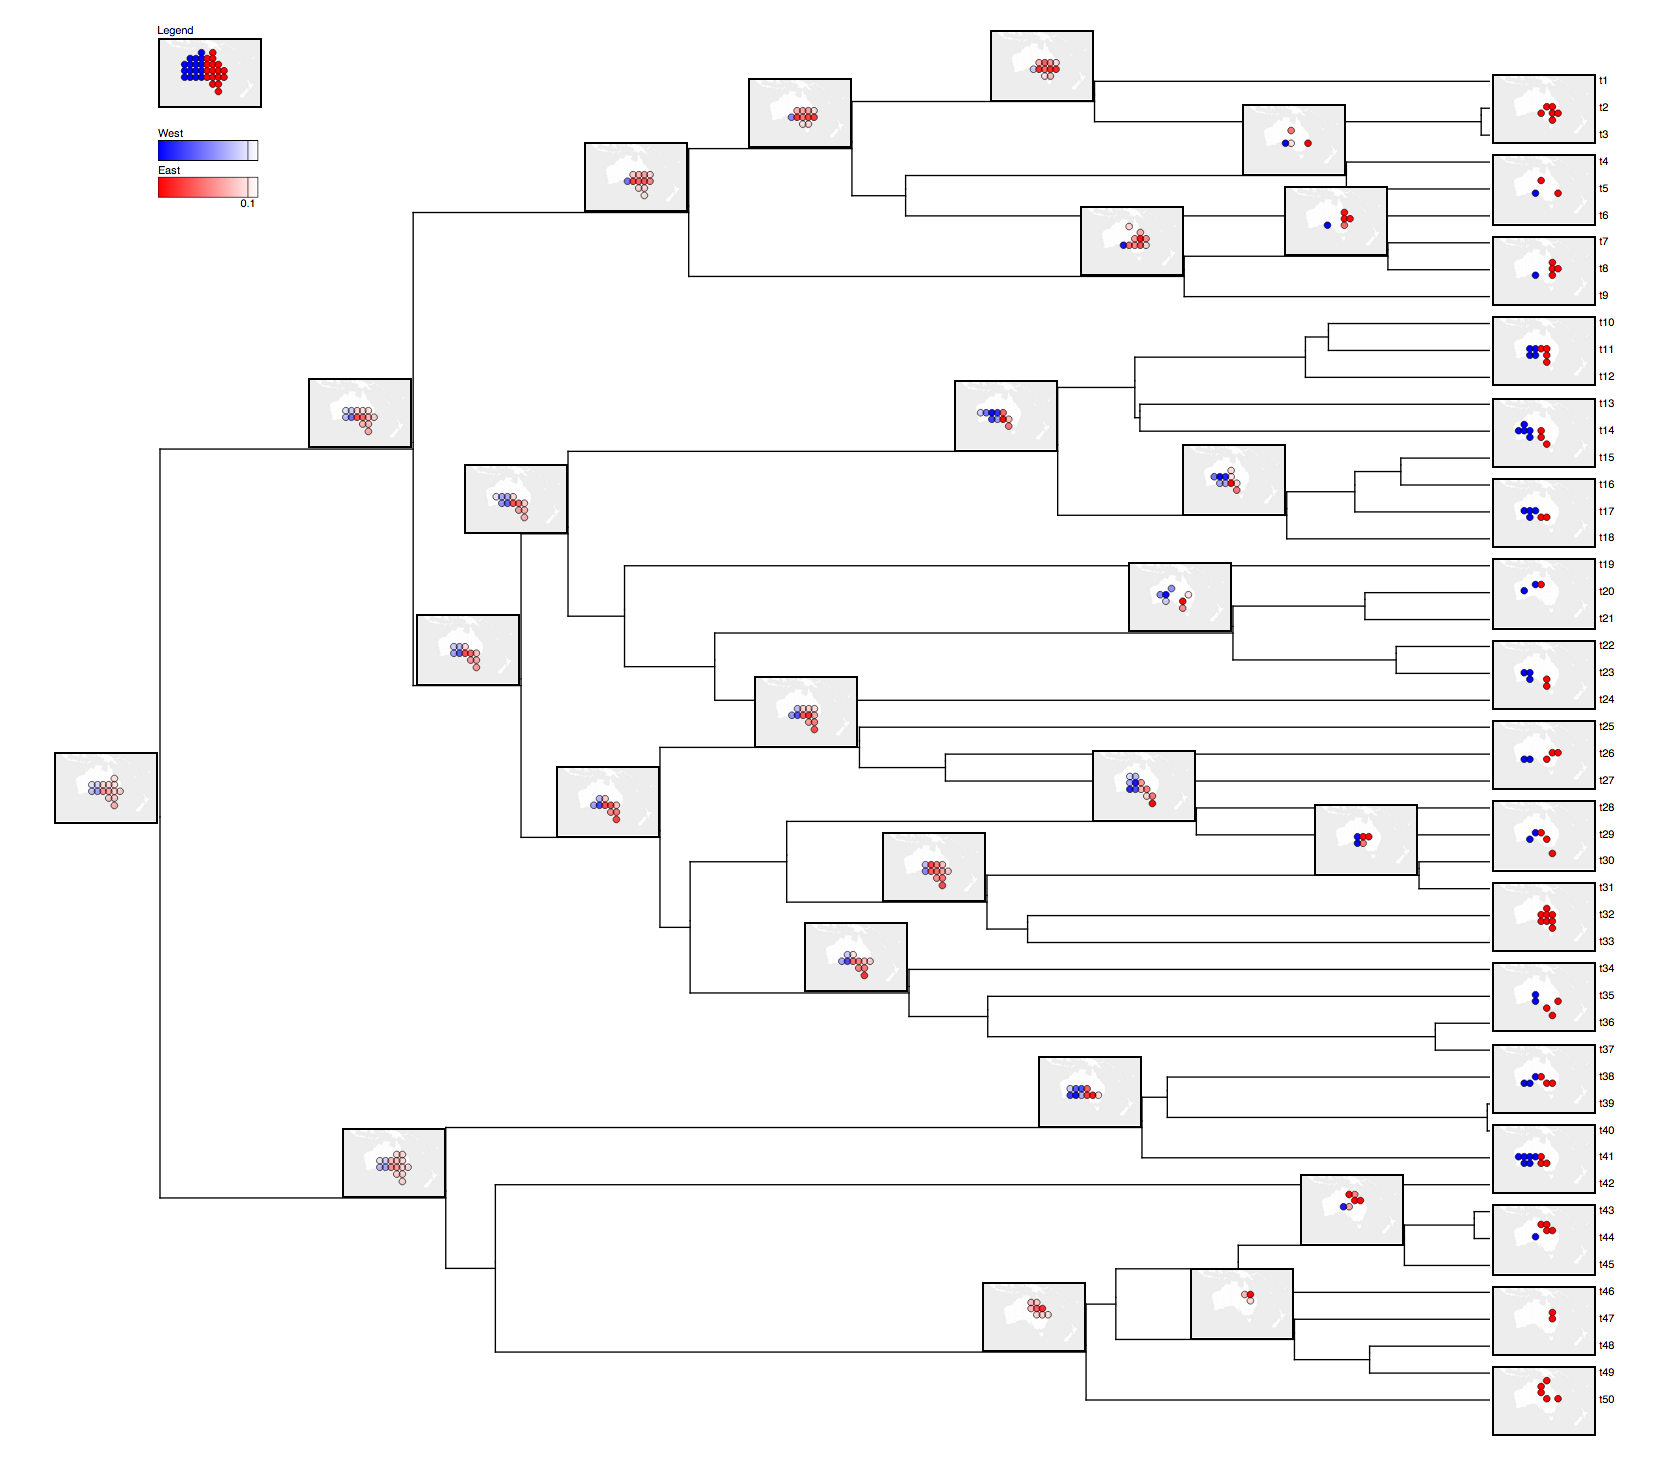
\includegraphics[width=4in]{figures/bayarea-fig}
\end{figure}

The generated figure reports the marginal area probabilities for each node in the phylogeny with a miniature map.
Because of the limited real estate in the figure, you may only wish to show a subset of ancestral ranges.

\noindent \\ \impmark  Click unwanted ancestral ranges to delete them. \\

Depending on the purpose for the figure, you may wish to alter its size.
The \texttt{mapheight}, \texttt{mapwidth}, \texttt{canvasheight}, and \texttt{canvaswidth} settings give the height and widths for the node-maps and the entire figure, respectively.

If you would like to differentiate areas (e.g. East from West, as above), give an ordered list of colors using the \texttt{areacolors} setting.
Next, in the order areas appear in the $\texttt{GEO}$ block, provide \texttt{areatypes} a list of assigments to area types.
In the above example ``0'' corresponds to the 0th \texttt{areacolors} group, ``blue'', and ``1'' corresponds to the 1st group, ``red''.

\noindent \\ \impmark Add a new color as the third \texttt{areacolors} entry. Add ``Tasmania'' as a third entry to \texttt{areanames}. Change the last area in \texttt{areatypes} to equal 2. \\

We've seen that ancestral range reconstructions contain a great deal of uncertainty.
Filtering out low probability ranges may make your figure easier to interpret.
If the marginal probability of presence for a node-area pair is less than \texttt{minareaval}, it is not shown.
The probabilities and the threshold value are shown in the upper left corner.

After arranging your figure, you'll want to save it to file.
How to accomplish this varies across operating systems and web browsers.
Generally, the figure is most easily saved from the browser by printing the file to pdf.
In this case the image size is equal to the paper size.
If the standard $8.5 \times 11$ inch image is too small, you will need to create and apply a sufficiently large custom paper size.

% \bibliography{bayes}

\newpage
\begin{sidewaysfigure}
\centering
\includegraphics[width=9in]{figures/bg_mol_dag}
\caption{Joint inference of range and molecular data. This figure explodes the module components in Figure \ref{fig:bm_mod}}
\label{fig:bm_dag}
\end{sidewaysfigure}

\end{document}

%{\it If you want to construct your own data matrix, I'll go over these topics below: collecting species occurrence data, identifying the total geographic region to include for analysis, and discretizing the geography into areas.}
%
%\subsubsection{Collecting species occurrence data}
%
%Species occurrence data minimally reports the latitude and longitude of a species of interest.
%For our analysis, a species is present in an area so long as that area contains a single occurrence record.
%For large areas, presence-absence characters are fairly robust to small measurement errors in geographical coordinates or imperfect sampling.
%[ I expect taxon sampling to be rel. unbiased since all biodiversity recorded per ``area''. ]
%I recommend querying the Global Biodiversity Information Facility (GBIF) database for a preliminary species occurrence dataset.
%
%[ Query georeference data ]
%Steps...
%
%[ Note gross outliers ]
%Some occurrence data may refer to museum or zoo specimens, or may be entirely erroneous (e.g. set to the default (latitude, longitude) of (0$^\circ$,0$^\circ$).
%
%[ Download data ]
%
%The default GBIF species occurrence query results are stored in the tab-delimited file, occurrence.txt.
%Using your favorite scripting language, you can easily extract the list of geographical coordinates per species.
%Because species names vary slightly between GBIF submissions, you should also take care to combine mismatched entries.
%Here is an example of the extracted (and cleaned) species occurrence data contained in occurrence.txt.
%
%\begin{framed}
%\begin{lstlisting}
%Canis lupus	-23.57222	132.78139
%Canis lupus	-13.75433	136.85133
%Canis aureus	33.06980	35.28452
%Canis aureus	32.02343	35.51647
%Canis latrans	45.89355	-69.99026
%...
%\end{lstlisting}
%\end{framed}
%
%Species with few or no GBIF occurrence records should be considered suspicious and supplemented with occurrence data reported in the scientific literature or (if applicable) taxon-specific biodiversity databases.
%
%So your work is useful, wait until after constructing the presence-absence data matrix to assess whether additional species occurrence records are required.
%
%\subsubsection{Identifying the total geographic region}
%
%Here we'd like to identify the geographic region(s) on Earth that extant and ancestral taxa may have occupied.
%For example, if you are studying purely terrestrial species, you may wish to exclude regions that contain no land.
%These regions will later be discretized into areas, then assigned presence-absence range data from the species occurrence records.
%The region(s) should minimally envelope all species occurrence data.
%
%[ Image ]
%
%You should consider two things before choosing to exclude certain regions from the analysis.
%First, is the region intermediate to the ranges of extant taxa?
%For instance, if sister taxa are endemic to North and South America respectively, then Central America may be considered for omission.
%However, this would forbid ancestral ranges from passing through the omitted region and greatly affect inference.
%Second, is the region 
%The range evolution model assumes a taxon is extinct when it is absent in all areas in the analysis.
%Extinction is always correctly considered when the set of areas covers the entire globe.
%
%\subsubsection{Discretizing the geography into areas}
%
%Geographic space is inherently continuous, so discretizing the geography into areas is a somewhat arbitrary process.
%Not much research has been done exploring how to best declare areas, so this section will introduce various strategies you may wish to consider.
%
%[ Image ]
%
%{\it Natural discretization.}
%Some regions are clearly discretized into areas, such as island archipelagos.
%Other regions contain suggested areas, such as those delimited by mountain ranges and bodies of water.
%Dispersal barriers will depend on the life history traits of your study taxa.
%Marking islands with presence-absence characters is quite easy while determining whether a point is within a polygon on the surface of a sphere is a more challenging problem in geometry.
%
%{\it Published discretization.}
%Biogeographic methods have defined areas in a variety of ways, using area cladograms, areas of endemism, etc.
%It may be tempting to use areas from previous biogeographic analyses for a BayArea (or other) statistical biogeographic analysis, but be wary.
%For instance, if parsimony-uninformative areas are discarded, then the inference of range expansion and contraction rates will surely be affected, which directly affects the ancestral range reconstructions.
%
%{\it Uniform discretization.}
%If you are unable to apply a satisfying rationale to define your areas, you could apply a uniform discretization over the geography.
%This strategy will treat the Earth as a sphere then discretize it using geodesic tiling (equilateral triangles).
%In this approach, all areas are equal in size and shape.
%The symmetry of uniform discretization offers some aid to easily identify which species are present in which areas.
%The following Python script generates a geodesic tiling, excludes water (or land) areas, converts species occurrence data into presence-absence characters, and writes files for the data matrix and area coordinates (below).